% Master report: local section inputs in iteration4_BDAS/Report.
\documentclass[a4paper]{article}
% PACKAGES

\usepackage[
    top=1.7cm,
    bottom=1.7cm,
    left=1.9cm,
    right=1.9cm
]{geometry}

\usepackage{setspace}
\usepackage{graphicx}
\usepackage{float}
\usepackage{booktabs}
\usepackage{tabularx}
\usepackage{array}
\usepackage{enumitem}
\usepackage[hidelinks]{hyperref}
\usepackage{xurl}
\usepackage{pgfgantt}
\usepackage{longtable}
\usepackage{array}

\usepackage{xcolor}
% Allows LaTeX to break long URLs more easily
\Urlmuskip=0mu plus 1mu

\onehalfspacing
\setlength{\parindent}{0pt}
\setlength{\parskip}{5pt}
\setlength{\emergencystretch}{2em}

% APA 7 referencing
\usepackage{csquotes}
\usepackage[
    backend=biber,
    style=apa,
    sorting=nyt
]{biblatex}

\addbibresource{references.bib}

\title{
    \textbf{Iteration 4 BDAS Report}\\[0.4cm]
    \large A Data Mining Solution for Early Gallstone Prediction\\
    to Support Sustainable Healthcare
}

\author{
    Duong Nguyen\\
    Student UUID: dugn944\\
    University of Auckland
}

\date{13 October 2026}

\begin{document}
\maketitle
\tableofcontents
\newpage

% 1. INTRODUCTION
\section{Introduction}
Sustainable Development Goal 3 (SDG 3), \textit{Good Health and Well-Being} \ref{fig:global_challenges}, aims to improve health outcomes through prevention, early intervention, and access to effective healthcare services. Achieving this goal increasingly depends on the ability of healthcare systems to use available data efficiently and support evidence-based clinical decisions. Data mining and machine learning can contribute to this objective by identifying hidden patterns in routinely collected health information and supporting earlier detection of disease risk.

\begin{figure}[H]
    \centering
    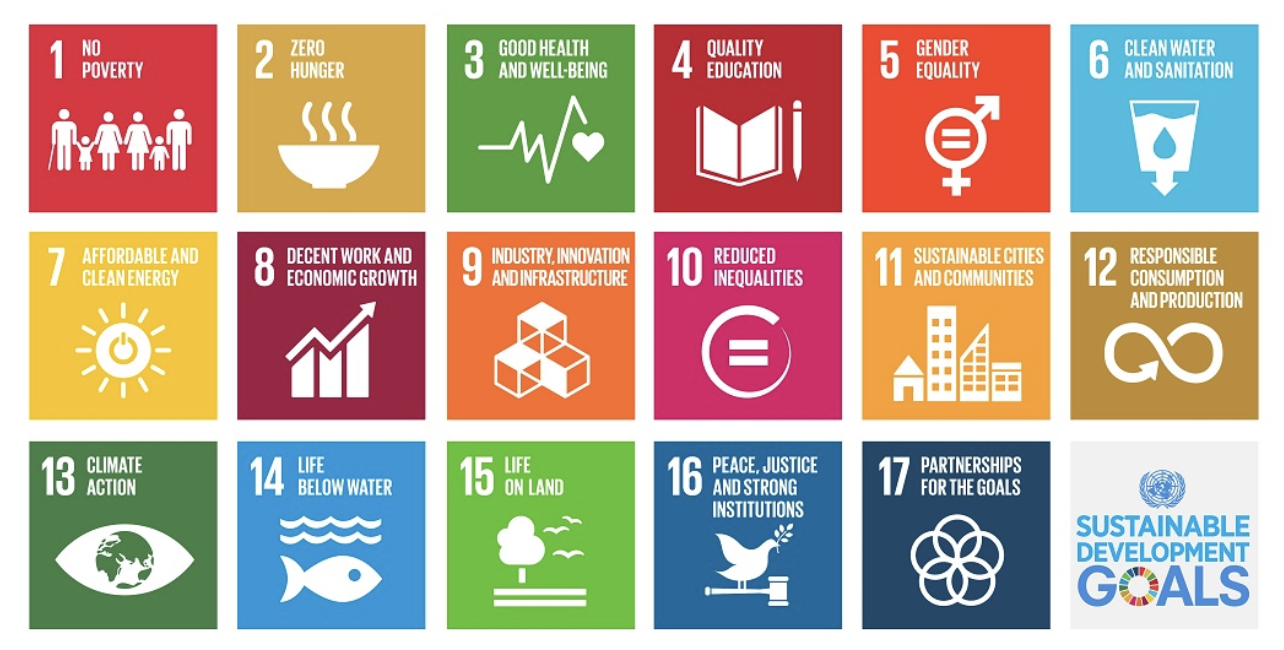
\includegraphics[width=0.8\linewidth]{media/SGD.png}
    \caption{17 Global Challenge for Government Transparency: The Sustainable Development Goals (SDG) 2030 Agenda }
    \label{fig:global_challenges}
\end{figure}

Gallstone disease is a common condition that may remain asymptomatic but can lead to complications such as acute cholecystitis, biliary obstruction, cholangitis, and pancreatitis \parencite{lammert2016gallstones,fujita2023guidelines}. Diagnosis generally relies on clinical assessment and abdominal ultrasonography. However, identifying high-risk individuals before complications occur may support earlier investigation and improve the efficient use of healthcare resources.

This project therefore develops a data-mining solution for the early prediction of gallstone disease using demographic, comorbidity, laboratory, and body-composition information. The Gallstone dataset contains records from 319 participants, including both patients with gallstones and control participants \parencite{esen2024early,uci2025gallstone}. Machine-learning models will be used to identify patterns associated with gallstone status and estimate individual disease risk.

The proposed solution is intended as a clinical decision-support tool rather than a replacement for medical diagnosis. By evaluating predictive performance, sensitivity, interpretability, and important risk factors, the project aims to demonstrate how data-driven healthcare can support preventive intervention, reduce avoidable complications, and improve resource allocation. In this way, the project contributes to a more proactive, efficient, and sustainable healthcare system aligned with the broader objectives of SDG 3.

The Iteration 4 submission now provides a native PySpark/Google Colab workflow distributed through GitHub. The saved native Spark execution supplies measured platform evidence; the earlier Python prototype remains available for controlled methodological comparisons, and new native feature-selection versions have separately recorded execution status.


% 2. BUSINESS AND SITUATION UNDERSTANDING
\section{Business and Situation Understanding}
\label{sec:business-understanding}
\subsection{Clinical background and motivation}

Gallstone disease (cholelithiasis) is a common hepatobiliary disorder in which solid deposits form within the gallbladder or biliary tract. Although many gallstones remain clinically silent, obstruction of the cystic or common bile duct can lead to biliary colic and complications such as acute cholecystitis, obstructive jaundice, cholangitis, and gallstone pancreatitis \cite{lammert2016gallstones,fujita2023guidelines}. A recent systematic review and meta-analysis estimated that approximately 6\% of the global population has gallstones, with prevalence varying substantially by sex and geographical region \cite{wang2024global}. The scale of the condition and the possibility of clinically important complications make the identification of individuals at increased risk a relevant preventive and diagnostic-support problem.

Gallstone formation is multifactorial rather than the result of a single abnormal measurement. Established or commonly reported associations include age, sex, obesity and body-fat distribution, metabolic abnormalities, dyslipidaemia, and diabetes \cite{lammert2016gallstones}. These relationships are relevant to the present dataset because its predictors combine demographic information, comorbidities, body-composition measurements, and routine laboratory markers. This creates an opportunity to investigate whether the joint pattern of routinely obtainable variables contains sufficient information to distinguish patients with and without gallstones.

In current clinical practice, abdominal ultrasonography remains a principal first-line imaging method for suspected gallstone disease, together with appropriate laboratory assessment \cite{easl2016guidelines,nice2014gallstone,fujita2023guidelines,gutt2020treatment}. Therefore, the purpose of the proposed machine learning system is \emph{not} to replace ultrasound or provide an autonomous diagnosis. Instead, the project treats prediction as a risk-stratification and decision-support problem: a model could estimate the probability of gallstone disease from non-imaging clinical information and thereby identify individuals who may warrant closer clinical assessment or confirmatory imaging.

This direction is supported by recent work applying machine learning to clinical and metabolic information. Salem et al.\ combined metabolomic and clinical predictors and demonstrated that nonlinear models can capture patterns associated with gallstone status \cite{salem2023ml}. More directly, Esen et al.\ introduced the dataset used in this project and reported that models based on bioimpedance and laboratory variables could distinguish gallstone cases from controls, with their strongest models reaching approximately 85\% accuracy and an area under the receiver-operating-characteristic curve (ROC--AUC) of about 0.85 \cite{esen2024early}. These results provide a useful benchmark, but they do not remove the need for careful validation, because the available sample is small and originates from a single clinical setting.

\subsection{Business and situation objectives}
\label{subsec:business-objectives}

The practical objective of this project is to develop and evaluate an interpretable early-risk prediction approach for gallstone disease using information that may already be available from routine clinical assessment, blood testing, and bioimpedance measurement. In a realistic healthcare workflow, the intended output would be a \emph{risk estimate} rather than a definitive diagnostic label. The model should help prioritise patients for further assessment while maintaining sufficient transparency for its predictions to be examined by a clinician.

Accordingly, the business/situation objectives are:

\begin{enumerate}
    \item Determine whether demographic, comorbidity, laboratory, and body-composition variables can provide useful early discrimination between patients with and without gallstones;
    \item Minimise clinically undesirable false-negative predictions, because a model that frequently classifies gallstone cases as low risk would have limited screening value;
    \item Identify the variables that contribute most strongly to predictions so that the resulting model remains interpretable and clinically reviewable; and
    \item Produce a reproducible proof-of-concept that can justify, but not substitute for, subsequent external clinical validation.
\end{enumerate}

For this iteration, business success is defined as evidence that the dataset can support a stable and interpretable risk-stratification model rather than evidence that the model is ready for clinical deployment. The analytical success criteria are therefore set as: (i) ROC--AUC of at least 0.80 under a validation procedure that keeps training and evaluation data separate; (ii) sensitivity/recall of at least 0.80 for the gallstone class at the selected decision threshold; (iii) performance superior to simple baselines such as majority-class prediction and standard logistic regression where possible; and (iv) reporting of calibration, confusion-matrix outcomes, and important predictors in addition to overall accuracy. These thresholds are project benchmarks chosen to make the data-mining goal measurable; they are not clinical guideline thresholds.

\subsection{Situation assessment}
\label{subsec:situation-assessment}

\subsubsection{Available resources and data}

The UCI Gallstone dataset originates from a prospective descriptive study conducted at the Internal Medicine Outpatient Clinic of Ankara VM Medical Park Hospital between June 2022 and June 2023 \cite{esen2024early,uci2025gallstone}. The source study initially considered 454 participants and excluded individuals who had previously undergone gallbladder surgery, leaving 319 participants for analysis: 161 with gallstones and 158 controls \cite{esen2024early}. The near-balanced outcome distribution is advantageous for a binary classification exercise because the model is not forced to learn from a severely under-represented positive class.

The dataset contains demographic variables, comorbidities, anthropometric measurements, bioimpedance measurements, hepatic-fat information, and routine laboratory results. Examples include age, sex, body mass index (BMI), diabetes, hyperlipidaemia, total body water, extracellular and intracellular water, body-fat and lean-mass measures, visceral fat measures, glucose, lipid markers, liver enzymes, creatinine, glomerular filtration rate, C-reactive protein (CRP), haemoglobin, and vitamin D \cite{esen2024early,uci2025gallstone}. The UCI repository describes the released data as having no missing values \cite{uci2025gallstone}; however, this must still be confirmed programmatically before modelling rather than assumed from documentation alone.

The dataset is computationally small and can be analysed on ordinary hardware. All development in this iteration will use Python, with reproducible scripts and notebooks used to record data validation, preprocessing, feature engineering, model fitting, and evaluation. The principal libraries are pandas and NumPy for data handling, scikit-learn for preprocessing, validation, and baseline models, and XGBoost and LightGBM for boosted-tree experiments.

\subsubsection{Requirements and assumptions}

Several requirements follow from the medical context. First, all predictor transformations must be fitted using training data only so that information from the evaluation set cannot leak into model development. Second, model performance must be reported with class-sensitive metrics---particularly sensitivity, specificity, precision, F1 score, ROC--AUC, and the confusion matrix---rather than accuracy alone. Third, model interpretation is required because a high-performing but opaque model would be difficult to justify as clinical decision support. Finally, the analysis should distinguish prediction from causal inference: an important feature may improve classification without being a causal determinant of gallstone formation.

A critical data-validation requirement is to verify the target encoding directly from the supplied dataset before analysis. The published study describes one numerical coding for gallstone presence, whereas the UCI repository documentation presents the class labels differently \cite{esen2024early,uci2025gallstone}. Similarly, repository metadata and the study description should be reconciled for the final number of observations. These discrepancies do not prevent modelling, but failure to resolve them could invert the target labels or create incorrect performance interpretation.

\subsubsection{Constraints, risks, and contingencies}

The principal constraint is sample size. With only approximately 319 participants and a relatively large number of candidate predictors, flexible models can overfit the training data. This risk will be reduced through stratified resampling, cross-validation, regularisation or restricted model complexity, and comparison with simpler baselines. Hyperparameter tuning and feature selection must occur inside the training/resampling process rather than on the full dataset.

A second constraint is external validity. The records come from a single hospital population in Ankara, and the observed relationships may not transfer directly to other countries, ethnic groups, age structures, or healthcare settings. Consequently, even strong internal validation results should be described as proof-of-concept evidence. External validation on an independent cohort would be required before clinical use.

A third risk concerns measurement availability. Some variables, particularly detailed bioimpedance measurements, may not be collected in every routine clinical setting. To address this, the project should compare a full-feature model with a reduced model based on more routinely available demographic and laboratory variables. If predictive performance remains similar, the reduced model may provide greater practical value.

Other risks include correlated body-composition variables, unstable feature importance, hidden coding errors, and optimistic results caused by repeated experimentation on the same test data. The contingency plan is to preserve a clear evaluation protocol, report uncertainty across resamples, investigate highly correlated variables, and avoid claiming that a small improvement in a single metric represents clinically meaningful superiority.

\subsection{Data-mining goals}
\label{subsec:data-mining-goals}

The data-mining task is a supervised binary-classification problem in which gallstone status is the target variable. The immediate technical goals are to:

\begin{enumerate}
    \item Audit variable types, ranges, coding, duplicates, and missing values;
    \item Explore relationships between gallstone status and demographic, metabolic, laboratory, and body-composition predictors;
    \item Establish interpretable baselines using logistic regression and a simple tree-based model;
    \item Compare a limited set of nonlinear classifiers such as random forest and gradient boosting using consistent resampling;
    \item Tune decision thresholds with particular attention to sensitivity and false-negative errors;
    \item Assess probability calibration in addition to discrimination;
    \item Evaluate model behaviour across clinically relevant subgroups, especially sex and age groups where sample size permits; and
    \item Use interpretable feature-attribution or model-specific importance methods to identify variables that consistently contribute to predictions.
\end{enumerate}

These goals align directly with the business objective: the model is useful only if it can identify higher-risk individuals with acceptable sensitivity, provide a meaningful probability estimate, and explain the factors contributing to that estimate. The strongest model will therefore not automatically be the model with the highest raw accuracy; model selection will consider discrimination, sensitivity, calibration, stability, and interpretability together.

\subsection{Project plan for the current iteration}
\label{subsec:project-plan}

Table~\ref{tab:iteration-plan} summarises the iteration running from 21 September to 16 October 2026. Development is organised around a common Python evaluation framework so that the baseline, data-centric, and model-centric strategies can be compared fairly using the same data partitions and metrics.

\begin{table}[htbp]
\centering
\caption{Iteration plan for PySpark development and evaluation, 21 September--16 October 2026; date labels and vertical guides use two-day intervals.}
\label{tab:iteration-plan}
\begin{tabularx}{\textwidth}{p{2.7cm} X X}
\toprule
\textbf{Dates} & \textbf{Main activities} & \textbf{Expected output} \\
\midrule
21--23 September & Confirm the business objective and success criteria; audit target coding, variable types, missing values, duplicates, ranges, and provenance in Python. & Validated problem statement, data dictionary, and data-quality log. \\
24--26 September & Complete exploratory analysis and implement a leakage-safe Python pipeline with fixed stratified 70/30 partitions and repeated seeds; establish logistic-regression and tree baselines. & Reproducible baseline workflow, saved split membership, and benchmark metrics. \\
27 September--3 October & Apply the \emph{data-centric strategy}: correct data-quality issues, assess transformations and outliers, engineer clinically meaningful features, compare full and reduced feature sets, and perform feature selection within cross-validation. & Audited feature sets and evidence of whether data improvements increase validation performance and stability. \\
27 September--6 October & In parallel, apply the \emph{model-centric strategy}: compare logistic regression, random forest, XGBoost, LightGBM, and stacking; tune promising models without accessing the test set. & Tuned candidate models and a cross-validated comparison table. \\
7--10 October & Evaluate alternative validation strategies using five-seed stratified holdout with training-only three-fold cross-validation; assess threshold choice, calibration, sensitivity, specificity, ROC--AUC, F1, and log loss. & Robustness analysis showing the effect of evaluation strategy and decision threshold. \\
11--13 October & Conduct error analysis, subgroup checks, feature-importance analysis, and comparison of data-centric, model-centric, and combined strategies. & Error profiles, interpretation outputs, and a defensible preferred approach. \\
14--16 October & Re-run the selected workflow, verify reproducibility, consolidate results and future work, and finalise the report and recommendations. & Reproducible Python artefacts and final iteration report. \\
\bottomrule
\end{tabularx}
\end{table}

\subsubsection{Development and data-mining plan}
The current iteration is scheduled from 21 September to 16 October 2026. Development uses native PySpark for the submitted extension, with the earlier Python prototype retained for comparison. The work begins with a reproducible
baseline and then separates improvement activities into two complementary
strategies. The data-centric strategy improves the quality and representation
of the input data through validation, transformation, feature engineering,
feature selection, and reduced-feature experiments. The model-centric strategy
holds the prepared data and evaluation rules constant while comparing model
families, hyperparameters, ensembles, calibration, and classification
thresholds. A final combined strategy uses only improvements supported by
validation evidence.

Figure~\ref{fig:gantt-iteration} presents the project timeline. The same saved
data partitions and metrics will be used across strategies to ensure that any
observed improvement is attributable to the tested change rather than to a
different evaluation setup.

\begin{figure}[H]
\centering
\resizebox{\textwidth}{!}{%
\begin{ganttchart}[
    hgrid,
    vgrid={draw=none,dotted},
    time slot format=isodate,
    title/.style={fill=gray!20},
    title label font=\bfseries\small,
    bar label font=\small,
    group label font=\bfseries\small,
    bar/.style={fill=blue!45},
    group/.style={fill=blue!70},
    milestone/.style={fill=red},
    x unit=0.36cm,
    y unit chart=0.55cm,
    y unit title=0.55cm
]{2026-09-21}{2026-10-16}

% Timeline
\gantttitle{September 2026}{10}
\gantttitle{October 2026}{16} \\
\gantttitlelist{21,23,...,29}{2}
\gantttitlelist{1,3,...,15}{2} \\

% Phase 1
\ganttgroup{Phase 1: Problem and Data Validation}
    {2026-09-21}{2026-09-23} \\

\ganttbar{Validate objective, target, variables, and provenance}
    {2026-09-21}{2026-09-23} \\

% Phase 2
\ganttgroup{Phase 2: Python Baseline and Evaluation Design}
    {2026-09-24}{2026-09-27} \\

\ganttbar{EDA, saved splits, pipelines, and baselines}
    {2026-09-24}{2026-09-27} \\

% Phase 3
\ganttgroup{Phase 3: Parallel Strategy Development}
    {2026-09-27}{2026-10-06} \\

\ganttbar[bar/.append style={fill=teal!55}]{Data-centric: standardization, CART/RFE, 20/10 fields}
    {2026-09-27}{2026-10-03} \\

\ganttbar[bar/.append style={fill=orange!65}]{Model-centric: native Spark models and training CV}
    {2026-09-27}{2026-10-06} \\

% Phase 4
\ganttgroup{Phase 4: Strategy Evaluation}
    {2026-10-06}{2026-10-10} \\

\ganttbar{Five-seed holdout, training CV and metrics}
    {2026-10-06}{2026-10-10} \\

% Phase 5
\ganttgroup{Phase 5: Error Analysis and Strategy Selection}
    {2026-10-10}{2026-10-13} \\

\ganttbar{Errors, subgroups, interpretation, and comparison}
    {2026-10-10}{2026-10-13} \\

% Phase 6
\ganttgroup{Phase 6: Reproducibility and Reporting}
    {2026-10-14}{2026-10-16} \\

\ganttbar{Re-run workflow and finalise report}
    {2026-10-14}{2026-10-16} \\

\ganttmilestone{Current iteration completed}
    {2026-10-16}

\end{ganttchart}%
}
\caption{Spark development and evaluation plan for the current gallstone
prediction iteration, 21 September--16 October 2026; date labels and vertical guides use two-day intervals.}
\label{fig:gantt-iteration}
\end{figure}

The baseline strategy provides the reference result against which subsequent
changes are assessed. In the data-centric stage, models are deliberately kept
stable while changes to data quality, transformations, engineered variables,
and feature subsets are evaluated. In the model-centric stage, the selected
data representation is held stable while algorithms and hyperparameters are
varied. Preprocessing and feature selection remain inside each resampling fold
to prevent leakage. Repeated holdout evaluation measures variation across
partitions. Three-fold cross-validation within each training partition supplies tuning and algorithm-selection evidence. The preferred approach will be
selected using sensitivity, specificity, ROC--AUC, F1, calibration, stability,
interpretability, and implementation complexity rather than accuracy alone.

Figure~\ref{fig:python-project-pipeline} clarifies the experimental pipeline.
The untouched test partition is used only after the data-centric and
model-centric choices have been made from training-only cross-validation evidence.

\begin{figure}[H]
\centering
\resizebox{\textwidth}{!}{%
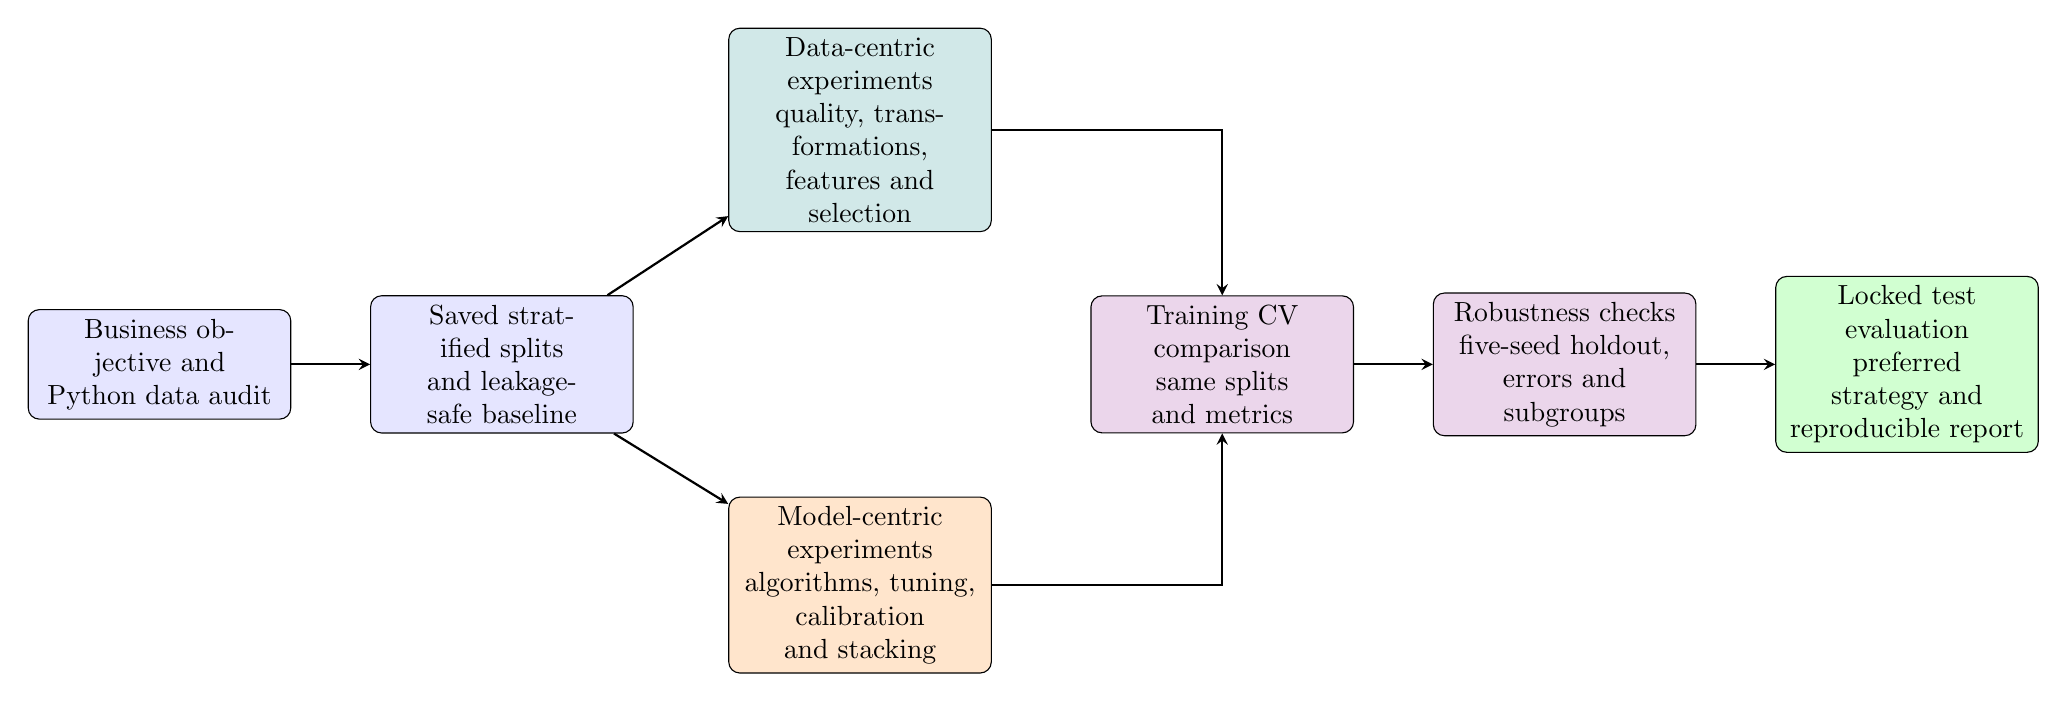
\begin{tikzpicture}[
    node distance=7mm and 10mm,
    stage/.style={draw, rounded corners, align=center, minimum height=9mm,
                  text width=3.1cm, fill=blue!10},
    data/.style={stage, fill=teal!18},
    model/.style={stage, fill=orange!20},
    decision/.style={stage, fill=violet!16},
    output/.style={stage, fill=green!18},
    arrow/.style={->, thick, >=stealth}
]
\node[stage] (audit) {Business objective and\\Python data audit};
\node[stage, right=of audit] (split) {Saved stratified splits\\and leakage-safe baseline};
\node[data, above right=8mm and 12mm of split] (datacentric)
    {Data-centric experiments\\quality, transformations,\\features and selection};
\node[model, below right=8mm and 12mm of split] (modelcentric)
    {Model-centric experiments\\algorithms, tuning,\\calibration and stacking};
\node[decision, right=58mm of split] (compare)
    {Training CV comparison\\same splits and metrics};
\node[decision, right=of compare] (robust)
    {Robustness checks\\five-seed holdout,\\errors and subgroups};
\node[output, right=of robust] (final)
    {Locked test evaluation\\preferred strategy and\\reproducible report};

\draw[arrow] (audit) -- (split);
\draw[arrow] (split) -- (datacentric);
\draw[arrow] (split) -- (modelcentric);
\draw[arrow] (datacentric.east) -| (compare.north);
\draw[arrow] (modelcentric.east) -| (compare.south);
\draw[arrow] (compare) -- (robust);
\draw[arrow] (robust) -- (final);
\end{tikzpicture}
}
\caption{Python project pipeline for comparing data-centric, model-centric,
and combined gallstone-prediction strategies.}
\label{fig:python-project-pipeline}
\end{figure}

\subsubsection{Report writing plan}
\label{subsec:report-writing-plan}

Report writing will be carried out progressively throughout the current
iteration rather than being postponed until the modelling work is complete.
Early sections describing the problem, dataset, and methodology will be
drafted while the corresponding analytical tasks are being completed.
Results, discussion, future work, and recommendations will then be added as
model outputs become available. This approach allows the report to be updated continuously and reduces the risk of documentation being disconnected from the implemented analysis.

Figure~\ref{fig:gantt-report-writing} presents the report-writing schedule for
21 September--16 October 2026.

\begin{figure}[H]
\centering
\resizebox{\textwidth}{!}{%
\begin{ganttchart}[
    hgrid,
    vgrid={draw=none,dotted},
    time slot format=isodate,
    title/.style={fill=gray!20},
    title label font=\bfseries\small,
    bar label font=\small,
    group label font=\bfseries\small,
    bar/.style={fill=green!45},
    group/.style={fill=green!70},
    milestone/.style={fill=red},
    x unit=0.36cm,
    y unit chart=0.55cm,
    y unit title=0.55cm
]{2026-09-21}{2026-10-16}

% Timeline
\gantttitle{September 2026}{10}
\gantttitle{October 2026}{16} \\
\gantttitlelist{21,23,...,29}{2}
\gantttitlelist{1,3,...,15}{2} \\

% Planning
\ganttgroup{Report Planning and Structure}
    {2026-09-21}{2026-09-23} \\

\ganttbar{Define report structure and section outline}
    {2026-09-21}{2026-09-22} \\

\ganttbar{Organise references and supporting materials}
    {2026-09-22}{2026-09-23} \\

% Introduction
\ganttgroup{Introduction and Problem Definition}
    {2026-09-23}{2026-09-27} \\

\ganttbar{Draft background and motivation}
    {2026-09-23}{2026-09-24} \\

\ganttbar{Write problem statement and objectives}
    {2026-09-25}{2026-09-26} \\

\ganttbar{Write project scope and success criteria}
    {2026-09-27}{2026-09-27} \\

% Data and Methodology
\ganttgroup{Data and Methodology}
    {2026-09-27}{2026-10-03} \\

\ganttbar{Document dataset and variables}
    {2026-09-27}{2026-09-28} \\

\ganttbar{Write data quality and EDA section}
    {2026-09-29}{2026-09-30} \\

\ganttbar{Document preprocessing and evaluation design}
    {2026-10-01}{2026-10-01} \\

\ganttbar{Describe baseline and candidate models}
    {2026-10-02}{2026-10-03} \\

% Results
\ganttgroup{Results}
    {2026-10-04}{2026-10-10} \\

\ganttbar{Prepare model performance tables}
    {2026-10-04}{2026-10-06} \\

\ganttbar{Prepare figures and visualisations}
    {2026-10-06}{2026-10-07} \\

\ganttbar{Write model comparison results}
    {2026-10-08}{2026-10-09} \\

\ganttbar{Write threshold and calibration results}
    {2026-10-10}{2026-10-10} \\

% Discussion
\ganttgroup{Discussion and Interpretation}
    {2026-10-10}{2026-10-13} \\

\ganttbar{Interpret predictive performance}
    {2026-10-10}{2026-10-10} \\

\ganttbar{Discuss feature importance and clinical relevance}
    {2026-10-11}{2026-10-12} \\

\ganttbar{Write future work and next iterations}
    {2026-10-13}{2026-10-13} \\

% Finalisation
\ganttgroup{Finalisation}
    {2026-10-14}{2026-10-16} \\

\ganttbar{Write conclusion and recommendations}
    {2026-10-14}{2026-10-14} \\

\ganttbar{Review consistency, citations, tables, and figures}
    {2026-10-14}{2026-10-15} \\

\ganttbar{Proofread and finalise report}
    {2026-10-16}{2026-10-16} \\

\ganttmilestone{Final report completed}
    {2026-10-16}

\end{ganttchart}%
}
\caption{Day-to-day report-writing plan for the gallstone prediction project,
21 September--16 October 2026; date labels and vertical guides use two-day intervals.}
\label{fig:gantt-report-writing}
\end{figure}

The completion criterion for this iteration is therefore a transparent comparison of feasible predictive models and a defensible conclusion about whether this dataset supports early gallstone-risk stratification. Clinical deployment, treatment decisions, and replacement of diagnostic imaging are explicitly outside the scope of the present iteration.


% 3. DATA UNDERSTANDING
\section{Data understanding}
\label{sec:data-understanding}
\subsection{Initial Data Collection}
\label{subsec:initial-data-collection}

The dataset used in this project was obtained from the UCI Machine Learning Repository and originates from the clinical study conducted by \textcite{esen2024early}. The original data were collected prospectively from patients attending the Internal Medicine Outpatient Clinic of Ankara VM Medical Park Hospital, Turkey, between June 2022 and June 2023 \parencite{esen2024early,uci2025gallstone}.

The original study initially collected information from 454 participants. Records from individuals who had previously undergone gallbladder surgery were excluded, resulting in a final published dataset of 319 participants. Among these, 161 participants were diagnosed with gallstone disease and 158 formed the control group \parencite{esen2024early}. Data collection included demographic and clinical characteristics, comorbidities, laboratory test results, and body-composition measurements obtained through bioimpedance analysis. The resulting dataset contains 38 predictive attributes relating to factors such as age, BMI, diabetes, lipid profiles, liver-function markers, glucose levels, body water, muscle mass, and body-fat distribution/

No additional primary data were collected for the current project; therefore, this analysis represents secondary use of the published clinical dataset. The UCI repository reports no missing values. However, an issue identified during initial data collection and validation is an inconsistency in the published metadata: the repository description reports 319 participants, while one metadata field lists 320 instances. Consequently, the downloaded dataset's row count and target coding will be independently verified before further analysis.

The dataset was downloaded in tabular form and will be retained in its original form as a raw-data copy before any cleaning or transformation is performed.

\subsection{Data Description}
\label{subsec:data-description}

The dataset contains one binary target variable, \textit{Gallstone Status}, and 38 predictor variables covering demographic characteristics, comorbidities, anthropometric measurements, body-composition indicators, and laboratory measurements. The predictors include both categorical and numerical variables, allowing the project to investigate multiple clinical and physiological factors that may be associated with gallstone disease.

According to the dataset documentation, no missing values are reported. However, the variable types, class coding, ranges, and missing-value patterns will be independently verified during the data-quality assessment before modelling. In particular, categorical variables stored numerically will be converted to appropriate factor or categorical representations to prevent their codes from being interpreted as continuous quantities.

Table~\ref{tab:data-dictionary} summarises the variables contained in the dataset.

\begin{longtable}{
    p{4.0cm}
    p{1.3cm}
    p{1.6cm}
    p{1.4cm}
    p{5.0cm}
    p{1.0cm}
    p{1.2cm}
}
\caption{Data dictionary for the Gallstone dataset.}
\label{tab:data-dictionary} \\

\toprule
\textbf{Variable} &
\textbf{Role} &
\textbf{Type} &
\textbf{Demo.} &
\textbf{Description} &
\textbf{Units} &
\textbf{Missing} \\
\midrule
\endfirsthead

\multicolumn{7}{c}%
{{\tablename\ \thetable{} -- continued from previous page}} \\

\toprule
\textbf{Variable} &
\textbf{Role} &
\textbf{Type} &
\textbf{Demo.} &
\textbf{Description} &
\textbf{Units} &
\textbf{Missing} \\
\midrule
\endhead

\midrule
\multicolumn{7}{r}{{Continued on next page}} \\
\endfoot

\bottomrule
\endlastfoot

Gallstone Status
& Target & Binary & --
& Presence or absence of gallstones
& -- & No \\

Age
& Feature & Integer & Age
& Age of the participant
& years & No \\

Gender
& Feature & Categorical & Gender
& Gender of the participant
& -- & No \\

Comorbidity
& Feature & Categorical & --
& Number of concomitant medical conditions
& -- & No \\

Coronary Artery Disease (CAD)
& Feature & Binary & --
& Presence of coronary artery disease
& -- & No \\

Hypothyroidism
& Feature & Binary & --
& Presence of an underactive thyroid gland
& -- & No \\

Hyperlipidemia
& Feature & Binary & --
& Presence of elevated blood lipid levels
& -- & No \\

Diabetes Mellitus (DM)
& Feature & Binary & --
& Presence of diabetes mellitus
& -- & No \\

Height
& Feature & Integer & --
& Height of the participant
& -- & No \\

Weight
& Feature & Continuous & --
& Body weight of the participant
& -- & No \\

Body Mass Index (BMI)
& Feature & Continuous & --
& Weight relative to height
& -- & No \\

Total Body Water (TBW)
& Feature & Continuous & --
& Total amount of water in the body
& -- & No \\

Extracellular Water (ECW)
& Feature & Continuous & --
& Amount of water outside body cells
& -- & No \\

Intracellular Water (ICW)
& Feature & Continuous & --
& Amount of water contained within body cells
& -- & No \\

Extracellular Fluid/Total Body Water (ECF/TBW)
& Feature & Continuous & --
& Ratio of extracellular fluid to total body water
& -- & No \\

Total Body Fat Ratio (TBFR)
& Feature & Continuous & --
& Proportion of total body mass consisting of fat
& \% & No \\

Lean Mass (LM)
& Feature & Continuous & --
& Proportion of lean body mass
& \% & No \\

Body Protein Content (Protein)
& Feature & Continuous & --
& Estimated proportion of body protein
& \% & No \\

Visceral Fat Rating (VFR)
& Feature & Integer & --
& Rating of visceral fat surrounding internal organs
& -- & No \\

Bone Mass (BM)
& Feature & Continuous & --
& Estimated bone mass
& -- & No \\

Muscle Mass (MM)
& Feature & Continuous & --
& Estimated amount of muscle mass
& -- & No \\

Obesity
& Feature & Continuous & --
& Estimated degree of excess adiposity
& \% & No \\

Total Fat Content (TFC)
& Feature & Continuous & --
& Estimated total amount of body fat
& -- & No \\

Visceral Fat Area (VFA)
& Feature & Continuous & --
& Estimated area of visceral adipose tissue
& -- & No \\

Visceral Muscle Area (VMA)
& Feature & Continuous & --
& Estimated visceral muscle measurement
& kg & No \\

Hepatic Fat Accumulation (HFA)
& Feature & Categorical & --
& Degree of fat accumulation in the liver
& -- & No \\

Glucose
& Feature & Continuous & --
& Blood glucose level
& -- & No \\

Total Cholesterol (TC)
& Feature & Continuous & --
& Total blood cholesterol level
& -- & No \\

Low Density Lipoprotein (LDL)
& Feature & Continuous & --
& Low-density lipoprotein cholesterol level
& -- & No \\

High Density Lipoprotein (HDL)
& Feature & Continuous & --
& High-density lipoprotein cholesterol level
& -- & No \\

Triglyceride
& Feature & Continuous & --
& Triglyceride concentration in the blood
& -- & No \\

Aspartate Aminotransferase (AST)
& Feature & Continuous & --
& Liver enzyme measurement
& -- & No \\

Alanine Aminotransferase (ALT)
& Feature & Continuous & --
& Liver enzyme measurement
& -- & No \\

Alkaline Phosphatase (ALP)
& Feature & Continuous & --
& Enzyme associated primarily with liver and bone
& -- & No \\

Creatinine
& Feature & Continuous & --
& Indicator associated with kidney function
& -- & No \\

Glomerular Filtration Rate (GFR)
& Feature & Continuous & --
& Estimated kidney filtration rate
& -- & No \\

C-Reactive Protein (CRP)
& Feature & Continuous & --
& Marker associated with systemic inflammation
& -- & No \\

Hemoglobin (HGB)
& Feature & Continuous & --
& Concentration of oxygen-carrying haemoglobin
& -- & No \\

Vitamin D
& Feature & Continuous & --
& Blood vitamin D level
& -- & No \\

\end{longtable}

\subsubsection{Categorical Variable Coding}
\label{subsubsec:categorical-coding}

Several categorical variables are represented by integer codes in the raw dataset. These values represent categories rather than continuous numerical quantities and therefore require appropriate treatment during preprocessing. The documented class labels are:

\begin{itemize}
    \item \textbf{Gallstone Status:}
    0 = gallstones present;
    1 = gallstones absent.

    \item \textbf{Gender:}
    0 = male;
    1 = female.

    \item \textbf{Comorbidity:}
    0 = no comorbidities;
    1 = one comorbid condition;
    2 = two comorbid conditions;
    3 = three or more comorbid conditions.

    \item \textbf{Coronary Artery Disease:}
    0 = no;
    1 = yes.

    \item \textbf{Hypothyroidism:}
    0 = no;
    1 = yes.

    \item \textbf{Hyperlipidemia:}
    0 = no;
    1 = yes.

    \item \textbf{Diabetes Mellitus:}
    0 = no;
    1 = yes.

    \item \textbf{Hepatic Fat Accumulation (HFA):}
    0 = no fat accumulation;
    1 = Grade 1 (mild);
    2 = Grade 2 (moderate);
    3 = Grade 3 (severe);
    4 = Grade 4 (very severe).
\end{itemize}

Although these categories are encoded numerically, they do not all have the same statistical interpretation. Binary variables such as diabetes and coronary artery disease can be represented as indicator variables, whereas \textit{Comorbidity} and \textit{Hepatic Fat Accumulation} are ordinal variables because their categories represent increasing levels of severity or burden. Their treatment during modelling will therefore be determined explicitly during the data-preparation stage.

\subsection{Data exploration}
\label{subsec:data-exploration}
Exploratory data analysis (EDA) was conducted on the raw dataset before any transformation or model training. The purpose was to understand the distribution of the target variable, examine the characteristics of the predictors, identify potential outliers or skewed variables, and investigate relationships that may influence subsequent data preparation and modelling.

\subsubsection{Target Variable Distribution} Figure~\ref{fig:target-distribution} shows the distribution of the target variable, \textit{Gallstone Status}. Based on the documented class encoding, 0 represents the presence of gallstones and 1 represents the absence of gallstones.

\begin{figure}[H]
    \centering
    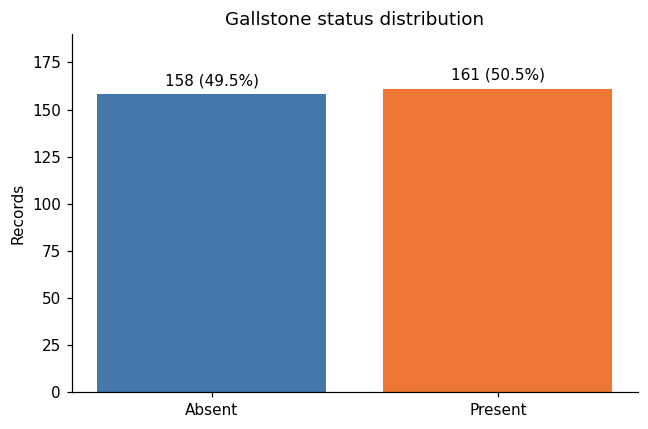
\includegraphics[width=.8\linewidth,keepaspectratio]{figures/pyspark_preparation/01_outcome_distribution.png}
    \caption{Gallstone status counts and percentages from the saved PySpark Colab visualization. Spark computed the counts; source code 0 means present and 1 means absent.}
    \label{fig:target-distribution}
\end{figure}

The dataset contains 161 participants with gallstones and 158 participants without gallstones. The two classes therefore account for approximately 50.5\% and 49.5\% of the observations, respectively. This indicates that the classification problem is almost perfectly balanced. This is an important characteristic for the subsequent modelling stage. Severe class imbalance is unlikely to be a major source of bias, and resampling techniques such as oversampling or undersampling are not immediately required. Nevertheless, stratified data partitioning will be used when dividing the observations into training and testing sets to preserve the approximately equal class proportions. Model evaluation will also consider sensitivity, specificity, F1-score and ROC-AUC rather than accuracy alone.

\subsubsection{Distribution of Continuous Features}
\label{sec:cont_distribution}

\begin{figure}[H]
    \centering
    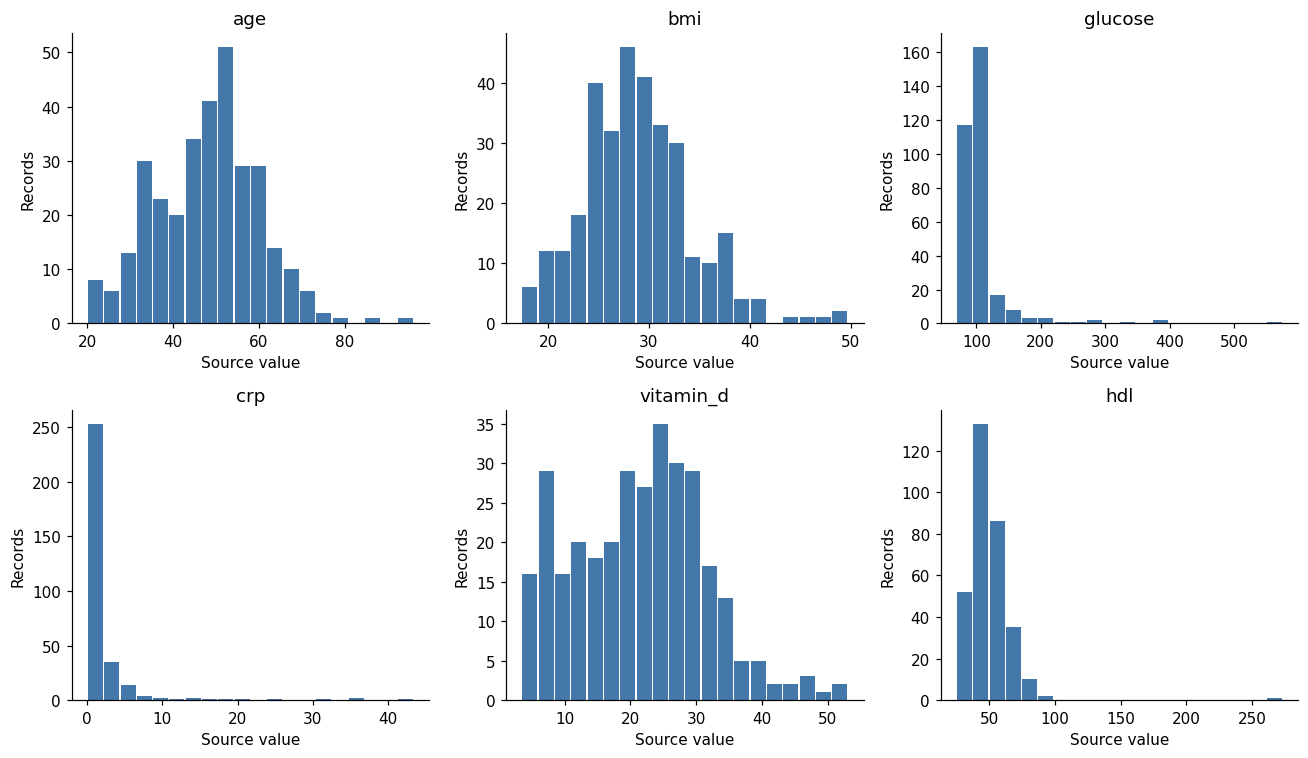
\includegraphics[width=1\linewidth,keepaspectratio]{figures/pyspark_preparation/03_continuous_distributions.png}
    \caption{Selected continuous distributions from the saved PySpark Colab visualization: age, BMI, glucose, CRP, vitamin D and HDL. Spark computed histogram counts. The discussion also covers the other source measurements reviewed in Iteration 3.}
    \label{fig:cont-dis}
\end{figure}

Figure~\ref{fig:cont-dis} presents the distributions of the continuous variables before any transformation or outlier treatment. The plots show considerable variation in distributional shape across the clinical and body-composition measurements.

Several variables, including age, height, BMI, extracellular water (ECW), lean mass, creatinine, haemoglobin, and visceral muscle area, display relatively smooth and approximately unimodal distributions. In contrast, variables such as glucose, triglyceride, AST, ALT, CRP, visceral fat rating (VFR), visceral fat area (VFA), and total fat content (TFC) show noticeable right-skewness, with most observations concentrated at lower values and a small number of substantially larger measurements.

The distributions also reveal several extreme observations, particularly in metabolic and laboratory variables. These values require further assessment during the data-quality stage to determine whether they represent valid clinical measurements or potential data errors. They will not be removed automatically, as unusual values may contain clinically meaningful information relevant to gallstone risk.

Overall, this exploration indicates that the predictors differ substantially in both scale and distribution. Consequently, standardisation and possible transformations of strongly skewed variables will be considered during data preparation, depending on the modelling technique used. The next stage of the analysis compares these predictors with \textit{Gallstone Status} to identify variables that may provide useful discriminatory information for the classification models.

\subsubsection{Distribution of categorical features and Association with Gallstone Status}
\label{subsubsec:categorical-distribution}

The categorical predictors were examined by comparing both the class counts and
the proportion of participants with gallstones within each category. This
provides an initial indication of whether particular categorical variables may
contain useful discriminatory information for the prediction task.

\begin{figure}[H]
    \centering
    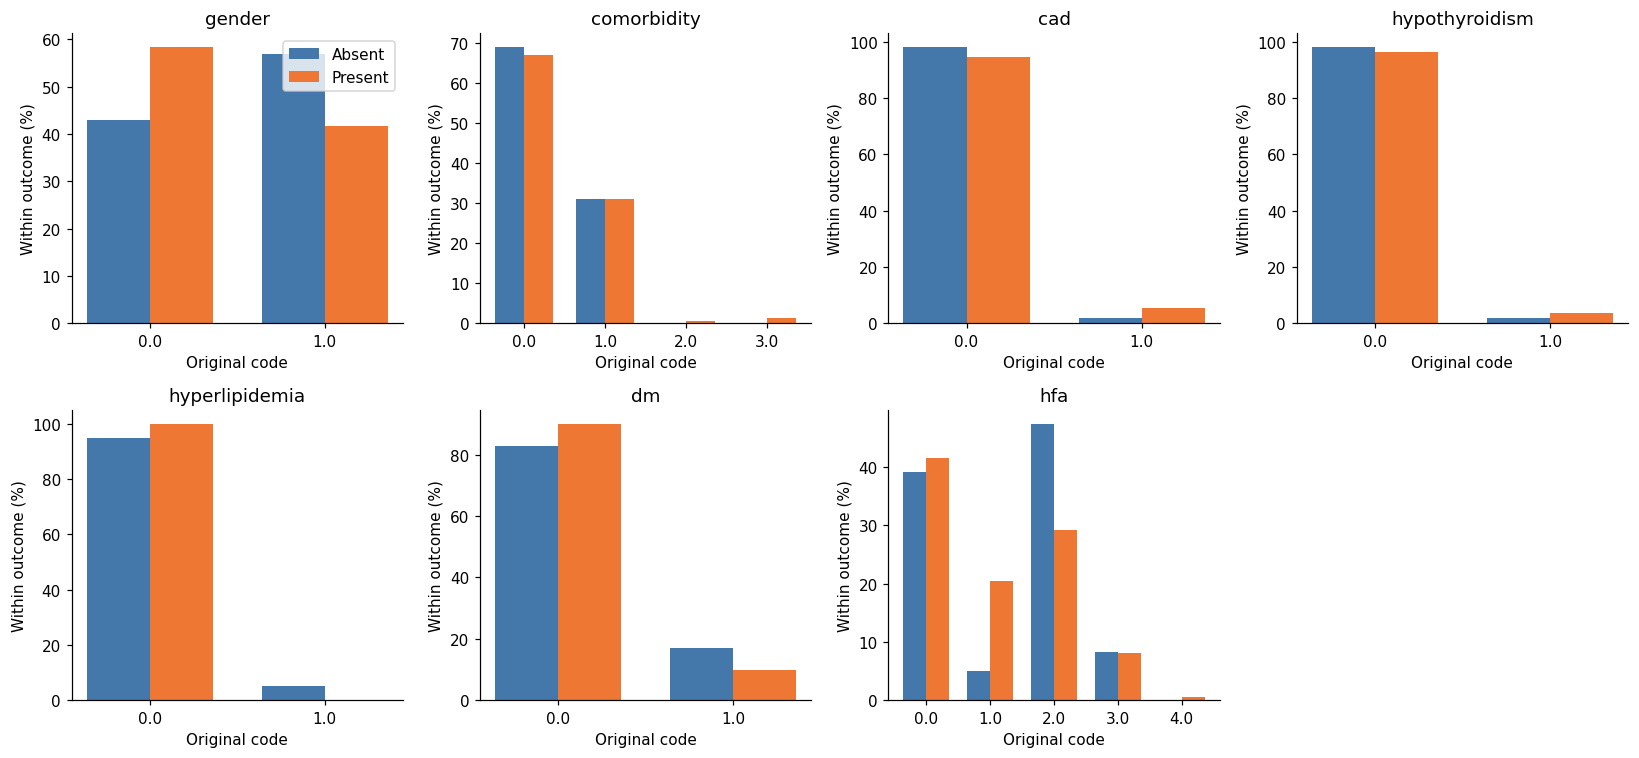
\includegraphics[width=.98\linewidth,keepaspectratio]{figures/pyspark_preparation/05_categorical_patterns.png}
    \caption{Original category-code distributions from the saved PySpark Colab visualization. Bars show percentages within each outcome group. Gallstone prevalence discussed in the analysis is calculated from the original category counts and uses a different denominator.}
    \label{fig:categorical-distribution}
\end{figure}

Figure~\ref{fig:categorical-distribution} suggests that the predictive signal
varies considerably across the categorical variables. Gender shows a moderate
difference between categories: the gallstone prevalence is approximately
42.0\% for category 0 and 57.3\% for category 1, indicating that gender may
provide some discriminatory information.

Diabetes mellitus (\texttt{dm}) also shows a potentially useful difference.
Gallstone prevalence is approximately 47.5\% among participants in category 0
compared with 62.8\% in category 1. A similar pattern is visible for
\texttt{hfa}, where prevalence varies across categories, most notably between
category 1 (19.5\%) and category 2 (61.5\%). This suggests that these variables
may contribute information useful for separating the two outcome classes.

In contrast, \texttt{comorbidity} shows little separation in the two major
categories, with gallstone prevalence close to 50\% in both. This indicates
limited univariate discriminatory value for this variable. \texttt{cad} and
\texttt{hypothyroidism} also show lower prevalence among category 1 than
category 0, although the number of observations in their positive categories is
small.

The strongest apparent difference is observed for \texttt{hyperlipidemia},
where all eight participants in category 1 have gallstones. However, this result
should be interpreted cautiously because the category contains very few
observations. Similar caution is required for rare levels of
\texttt{comorbidity} and \texttt{hfa}, where prevalence estimates are based on
only one or two participants and are therefore highly unstable.

Overall, the categorical EDA provides evidence of some class-related signal,
particularly for gender, diabetes mellitus, and selected HFA categories.
However, no single categorical predictor provides a sufficiently strong or
stable separation between participants with and without gallstones. The results
therefore support retaining these variables for multivariable modelling, where
their combined effects and interactions with continuous clinical and
body-composition measurements can be evaluated.


\subsubsection{Correlation Analysis}
\label{subsubsec:correlation}

Figure~\ref{fig:spearman-correlation} presents the Spearman correlationmatrix for the dataset. Spearman correlation was selected because several
continuous variables are skewed and contain extreme observations.

\begin{figure}[H]
    \centering
    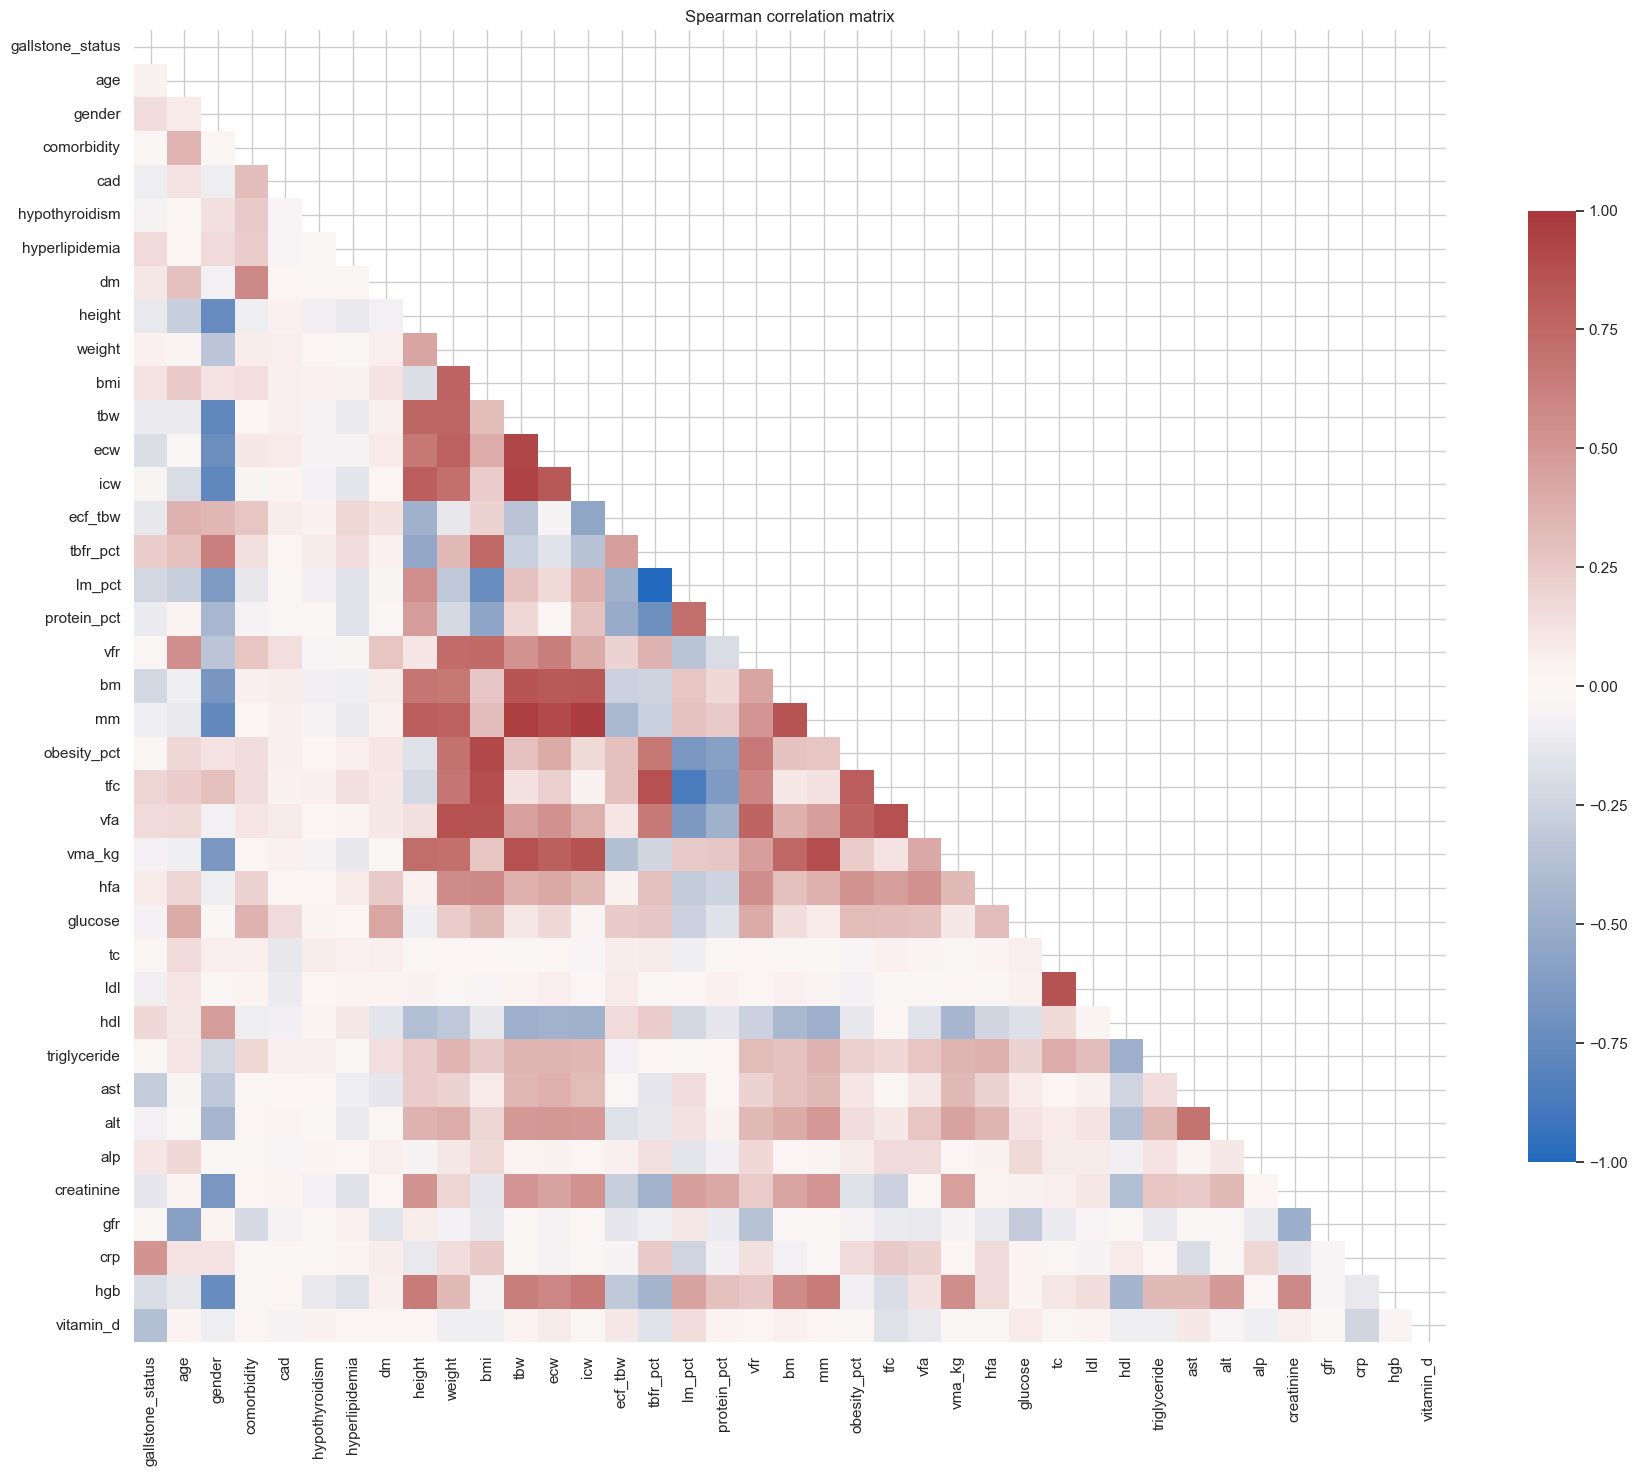
\includegraphics[width=0.75\textwidth]{media/correlation.png}
    \caption{Spearman correlation matrix for the Gallstone dataset visualization.}
    \label{fig:spearman-correlation}
\end{figure}

The matrix shows several groups of strongly related predictors. In particular, body-composition variables such as weight, BMI, TBW, ECW, ICW, muscle mass, body-fat measures, and visceral-fat measures show substantial correlation. Laboratory variables also contain related groups, including
TC-LDL, AST-ALT, and the inverse relationship between creatinine and GFR. These patterns indicate potential redundancy and multicollinearity among some predictors.

In contrast, individual correlations with \textit{Gallstone Status} are generally weaker. This suggests that gallstone status is unlikely to be explained by a single predictor and supports the use of multivariable classification models that combine demographic, body-composition, and
laboratory information.

These findings will guide the data-preparation stage. Highly correlated variables will be reviewed during feature selection, particularly for logistic regression, while tree-based models will also be considered because they are less sensitive to multicollinearity.


\subsubsection{Structure Among Body-Composition Variables}

Some body-composition variables, including total body water (TBW), bone mass (BM), and muscle mass (MM), appear to have broader or mildly multi-peaked distributions. This may indicate underlying differences between participant subgroups, for example differences in sex, body size, or body composition. At this stage, however, the univariate plots alone are insufficient to determine the cause. Furthermore, several predictors measure related physiological concepts. For example, BMI, TBFR, TFC, VFR and VFA all contain information relating to body fat or adiposity, while TBW, ECW and ICW describe different components of body watxer. Consequently, correlation analysis will be conducted in the next stage to determine whether some predictors contain highly overlapping information. Highly correlated variables will be reviewed before modelling to reduce unnecessary redundancy and potential multicollinearity, particularly for regression-based classifiers.


Overall, the EDA provides the foundation for the next data-preparation phase by identifying class balance, distributional characteristics, outliers, potentially informative predictors, and redundant variables. These findings will subsequently guide preprocessing, feature selection, model selection, and evaluation.

\subsection{Data Quality}
Data quality was assessed before any transformation or model development to ensure that errors in the raw data would not be carried into the predictive models. The verification focused on missing values, duplicate records, categorical coding, numerical ranges, and potential outliers.

\subsubsection{Missing Values and Completeness}
The dataset documentation reports no missing values, and this was confirmed during the initial inspection of the dataset. Therefore, no imputation was required at this stage. Nevertheless, missing-value checks will remain part of the preprocessing workflow to ensure that any values introduced during transformation or partitioning are detected before modelling.


\subsubsection{Potential Outliers and Data Quality Issues}
\label{sec:outliers}

\begin{figure}[H]
    \centering
    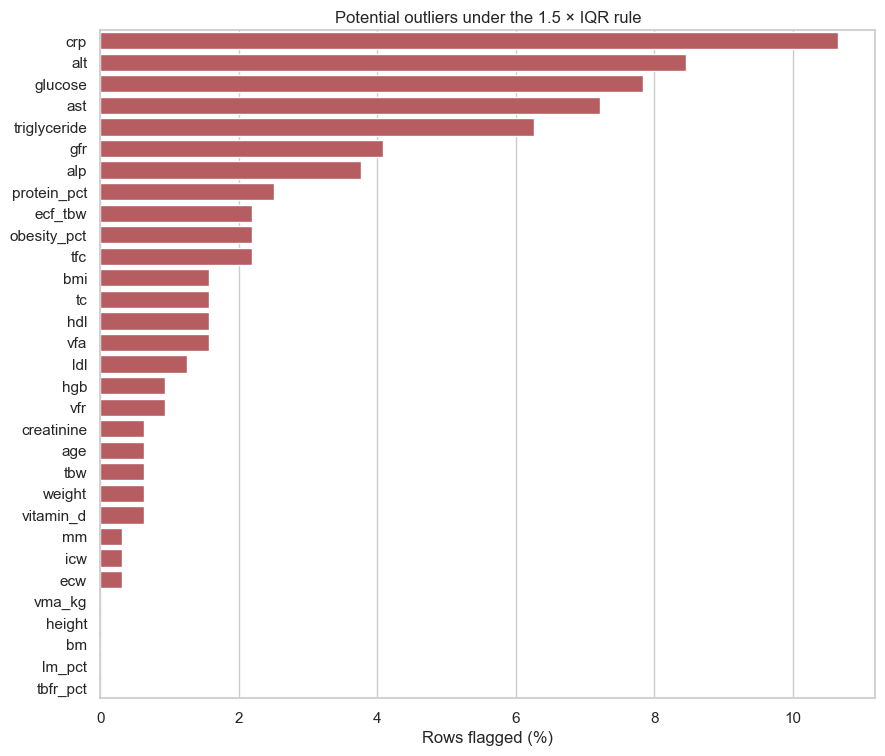
\includegraphics[width=\linewidth]{media/Outlier_Analysis.png}
    \caption{Outlier analysis using the 1.5$\times$IQR method.}
    \label{fig:outlier-analysis}
\end{figure}

Figure~\ref{fig:outlier-analysis} identifies several observations that require further investigation. Most notably, the \textit{Obesity} variable contains an extreme value of approximately 2000, which is substantially larger than the remaining observations. Given the magnitude of this difference, the value should be verified against the original dataset and variable definition to determine whether it represents a valid measurement, a unit inconsistency, or a data-entry error.

Potential upper-tail outliers are also observed in variables including glucose, HDL, triglyceride, AST, ALT, CRP, and intracellular water (ICW). However, observations identified by the 1.5$\times$IQR rule should not automatically be treated as erroneous, particularly in clinical data where extreme measurements may represent genuine patient conditions. Therefore, these observations will be reviewed during data preparation before any correction, transformation, or removal is applied.

Valid extreme observations will be retained where appropriate to preserve clinically meaningful variation in the dataset. Only values supported by evidence of coding, measurement, or data-entry errors will be considered for correction or exclusion. This approach reduces the risk of removing informative clinical cases and introducing bias into subsequent predictive models.


\subsubsection{Dimensionality Reduction Visualisation and Data Understanding}
\label{subsubsec:dimensionality_reduction}

Dimensionality-reduction techniques were used to obtain a more compact view of
the relationships among the continuous measurements and to assess whether
participants with and without gallstones exhibit distinct multivariate patterns.
Two complementary approaches were considered: Principal Component Analysis
(PCA) and t-distributed Stochastic Neighbor Embedding (t-SNE). PCA provides a
linear representation of the dominant sources of variance in the data, whereas
t-SNE is a nonlinear technique designed to preserve local neighbourhood
relationships in a low-dimensional representation
\parencite{vandermaaten2008tsne}.

\paragraph{Principal Component Analysis}

PCA was first applied to the continuous measurements to examine the main
directions of variation in the dataset. The first principal component (PC1)
explained 27.7\% of the total variance, while the second principal component
(PC2) explained a further 20.0\%. Together, the first two components therefore
accounted for approximately 47.7\% of the variance in the continuous feature
space.

\begin{figure}[H]
    \centering
    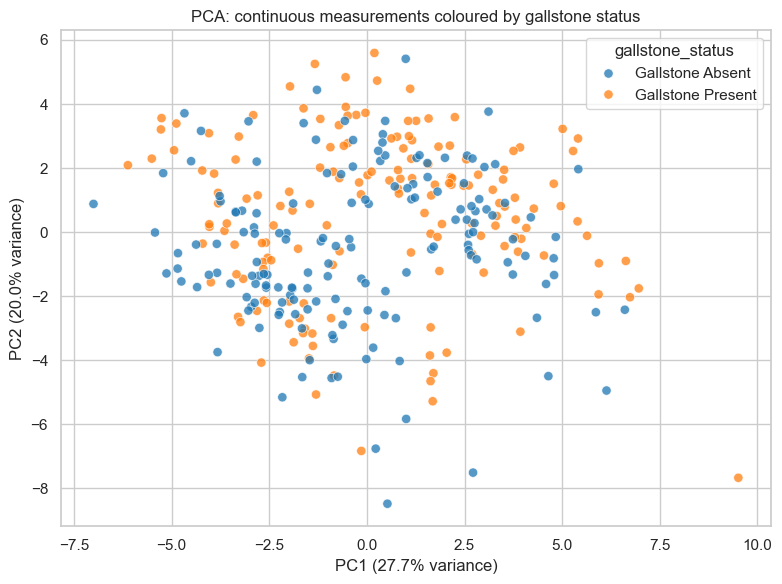
\includegraphics[
        width=0.76\linewidth,
        keepaspectratio
    ]{media/PCA.png}
    \caption{Two-dimensional PCA projection of the continuous measurements,
    coloured by Gallstone Status. PC1 and PC2 explain 27.7\% and 20.0\% of the
    total variance, respectively.}
    \label{fig:pca_projection}
\end{figure}

As shown in Figure~\ref{fig:pca_projection}, observations from the
\textit{Gallstone Present} and \textit{Gallstone Absent} groups overlap
substantially in the first two principal components. No distinct linear
separation between the two outcome groups is apparent. This indicates that the
largest sources of variation in the continuous measurements are not themselves
equivalent to the variation that separates gallstone status.

Nevertheless, the projection reveals meaningful structure within the
measurements. Participants are distributed across several regions of the PCA
space, suggesting heterogeneity in body-composition, anthropometric, and related
clinical characteristics. A small number of observations also lie relatively
far from the central concentration of the data. These observations are
consistent with the unusual or extreme measurements identified during the
earlier univariate exploration and were retained for further investigation
rather than being removed solely on the basis of their position in the PCA
projection.

To understand which variables contribute most strongly to the two principal
components, the corresponding PCA loadings were also examined.

\begin{figure}[H]
    \centering
    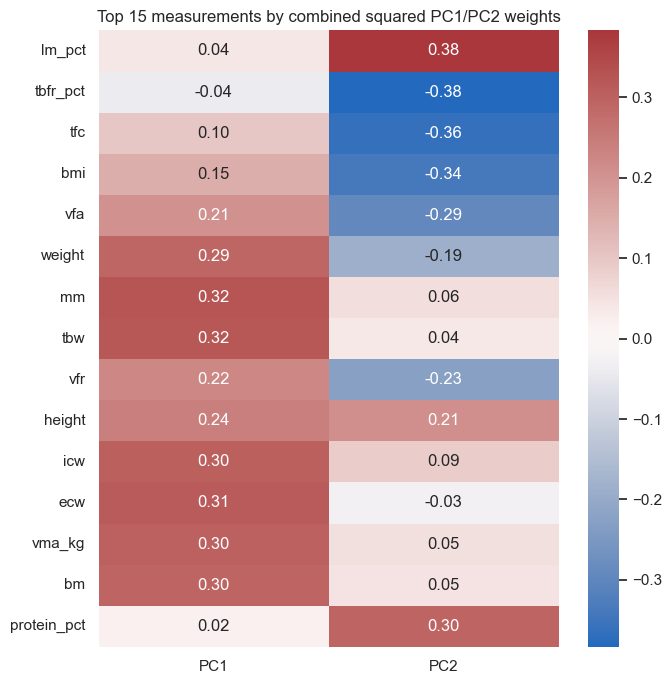
\includegraphics[
        width=0.62\linewidth,
        keepaspectratio
    ]{media/PCA_weight_measurement.png}
    \caption{Loadings of the 15 continuous measurements with the largest
    combined squared contributions to PC1 and PC2. Positive and negative values
    indicate the direction of association with each principal component.}
    \label{fig:pca_loadings}
\end{figure}

Figure~\ref{fig:pca_loadings} shows that PC1 is influenced primarily by several
body-size and body-composition measurements. Muscle mass (\texttt{mm}),
total body water (\texttt{tbw}), extracellular water (\texttt{ecw}),
intracellular water (\texttt{icw}), visceral muscle area
(\texttt{vma\_kg}), bone mass (\texttt{bm}), weight, and height all have
positive loadings on PC1. This suggests that PC1 broadly represents variation
associated with overall body size and lean/body-composition characteristics.

PC2 captures a different contrast. Lean-mass percentage
(\texttt{lm\_pct}) and protein percentage (\texttt{protein\_pct}) have strong
positive loadings, whereas total body-fat percentage (\texttt{tbfr\_pct}),
total fat content (\texttt{tfc}), BMI, visceral fat area (\texttt{vfa}), and
visceral fat rating (\texttt{vfr}) have negative loadings. PC2 can therefore be
interpreted as reflecting a contrast between lean-body composition and
fat-related measurements. These loading patterns provide additional insight into
the correlations among the original measurements and help explain the structure
observed in the PCA projection.

\paragraph{t-SNE Visualisation}

Because PCA represents only linear combinations of the original variables, a
nonlinear t-SNE analysis was additionally performed to examine whether local
neighbourhood structures could reveal patterns that were not visible in the PCA
projection. Multiple perplexity values were evaluated rather than relying on a
single t-SNE configuration.

\begin{figure}[H]
    \centering
    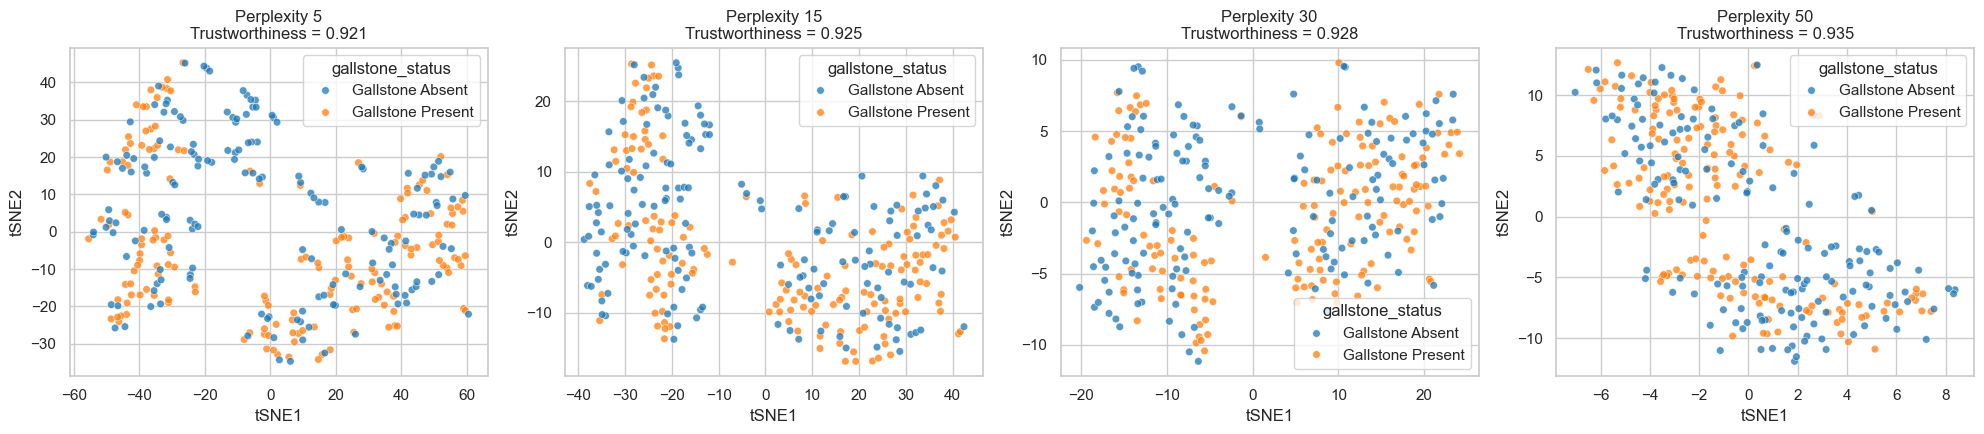
\includegraphics[
        width=\linewidth,
        keepaspectratio
    ]{media/TSNE_visualization.png}
    \caption{Two-dimensional t-SNE projections of the continuous measurements
    using perplexity values of 5, 15, 30, and 50. Points are coloured according
    to Gallstone Status. Trustworthiness scores are reported for each
    configuration.}
    \label{fig:tsne}
\end{figure}

Figure~\ref{fig:tsne} shows that the overall appearance of the t-SNE
representation changes as the perplexity parameter increases. Lower perplexity
values, particularly 5, emphasise very local neighbourhoods and produce a more
fragmented representation. At larger perplexities, the observations form
broader and more coherent structures.

The trustworthiness score increased from 0.921 at perplexity 5 to 0.935 at
perplexity 50, indicating that the higher-perplexity representations preserved
the original local neighbourhood relationships slightly more effectively.
However, the purpose of this metric is to assess preservation of neighbourhood
structure rather than separation of the target classes.

Across all perplexity settings, participants with and without gallstones remain
substantially intermixed. Although some local regions contain a greater
concentration of one class than the other, there is no stable class-specific
cluster or simple visual boundary that consistently separates
\textit{Gallstone Present} from \textit{Gallstone Absent}. The same general
conclusion is therefore observed in both the linear PCA representation and the
nonlinear t-SNE representations.


These findings suggest that gallstone status is unlikely to be explained by a
single dominant measurement or by a simple low-dimensional boundary. Instead,
the predictive information may be distributed across several demographic,
body-composition, metabolic, and biochemical variables and may involve
interactions or nonlinear relationships among them. This observation motivates
the subsequent comparison of multivariable classification models.

Importantly, both PCA and t-SNE were used here as exploratory tools for data
understanding rather than as measures of predictive performance. Visual overlap
between the classes does not imply that the target is unpredictable, since
discriminative information may exist in dimensions that are not represented by
the first two principal components or by the two-dimensional t-SNE embedding.
Model performance is therefore assessed separately using the validation and test
partitions.


% 4. DATA PREPARTION
\section{Data Preparation}
\label{sec:data-preparation}
The purpose of the data-preparation stage was to transform the raw Gallstone
dataset into a consistent, traceable, and modelling-ready dataset. Decisions
made during this stage were informed by the business objective, findings from
the exploratory analysis, data-quality checks, and the technical requirements
of the modelling pipeline.

All data-preparation procedures were implemented using an open-source Python
workflow. The main libraries used were \texttt{pandas} and \texttt{NumPy} for
data manipulation and validation, \texttt{SciPy} for statistical
transformations, \texttt{scikit-learn} for data partitioning and preprocessing,
and \texttt{Matplotlib} and \texttt{Seaborn} for diagnostic visualisation.

Using Python rather than a graphical modelling environment provides a
script-based and reproducible workflow in which each preprocessing operation can
be inspected, rerun, and consistently applied to subsequent modelling
experiments.


\subsection{Data Selection}
\label{subsec:data-selection}

The modelling dataset contains \textit{Gallstone Status} as the target variable
and the available demographic, comorbidity, body-composition, and laboratory
measurements as candidate predictors. Variables were initially retained rather
than removed solely on the basis of weak univariate relationships because the
exploratory analysis suggested that gallstone status may depend on combinations
of multiple patient characteristics.

Data selection was performed programmatically using Python. The dataset was
loaded into a \texttt{pandas DataFrame}, after which column names, data types,
unique values, distributions, and summary statistics were inspected. Candidate
predictors were retained when they had plausible clinical relevance and
sufficient data quality for subsequent modelling.

Variables containing unusual values, strong skewness, or high correlations with
other predictors were not immediately removed. Instead, these characteristics
were investigated during exploratory analysis and preprocessing. In particular,
highly correlated predictors were reviewed during feature selection because
multicollinearity may influence coefficient stability in models such as
logistic regression.

No patient-identifying information or variables without potential predictive
value were required for model development. Identifier fields used for data
traceability were retained during data processing but excluded from the feature
matrix supplied to the predictive models.


\subsection{Data Cleaning}
\label{subsec:data-cleaning}

Data cleaning was guided by the issues identified during the earlier
data-quality assessment. The Python workflow systematically evaluated missing
values, duplicated records, invalid categorical codes, numerical ranges, data
types, and potential extreme observations.

Completeness was assessed using functions such as
\texttt{DataFrame.isna()}, while duplicate observations and field-level
consistency were examined using standard \texttt{pandas} operations. Summary
statistics and value-frequency tables were also generated to identify
unexpected values and inconsistencies.

No missing values were identified in the original dataset; therefore, no
imputation was required before modelling. Nevertheless, missing-value checks
were retained as part of the preprocessing pipeline so that the workflow can
identify incomplete observations if the dataset is modified or extended in
future iterations.

Categorical variables were checked against their documented coding ranges.
Binary and ordinal fields stored numerically were treated according to their
clinical meaning rather than automatically interpreted as continuous
measurements.

Potential outliers were identified during exploratory analysis using the
1.5$\times$IQR rule:

\[
    \mathrm{Lower\ Bound} =
    Q_1 - 1.5(Q_3-Q_1),
\]

\[
    \mathrm{Upper\ Bound} =
    Q_3 + 1.5(Q_3-Q_1).
\]

Observations outside these limits were reviewed rather than automatically
removed. This distinction is important for clinical data because statistically
extreme observations may nevertheless correspond to genuine patient
measurements.

In particular, the unusually large observation identified in the
\textit{Obesity} variable was reviewed as a possible data-quality issue.
Similarly, extreme observations in glucose, triglyceride, AST, ALT, CRP, and
other laboratory measurements were retained when they represented plausible
clinical values. Records would only be corrected or excluded if there were
sufficient evidence of a coding, unit, or data-entry error.

Column names were also standardised programmatically to remove unnecessary
spaces and special characters and to provide consistent variable names
throughout the analysis.


\subsubsection{Cleaning and Sanity-Checking Workflow}

The data-cleaning process was implemented as a reproducible sequence of Python
operations. The main stages were:

\begin{enumerate}
    \item verify the number of observations and variables;
    \item inspect data types and expected variable roles;
    \item identify missing and blank values;
    \item detect duplicate observations;
    \item validate categorical coding ranges;
    \item examine descriptive statistics for continuous measurements;
    \item identify potential extreme observations;
    \item standardise column names and field representations; and
    \item confirm the dimensions and integrity of the resulting analytical
          dataset.
\end{enumerate}

This workflow provided explicit quality-control checkpoints while preserving the
original observations whenever no clear data-quality issue was present.

\subsubsection{Skewness Assessment and Transformation of Continuous Features}
\label{subsubsec:skewness-transformation}

The distributions of the continuous predictors were further examined using
sample skewness to identify variables with substantial departures from
symmetry. Absolute skewness values greater than or equal to 1 were treated as
an indication of strong skewness and were selected for further transformation
assessment.

\begin{figure}[H]
    \centering
    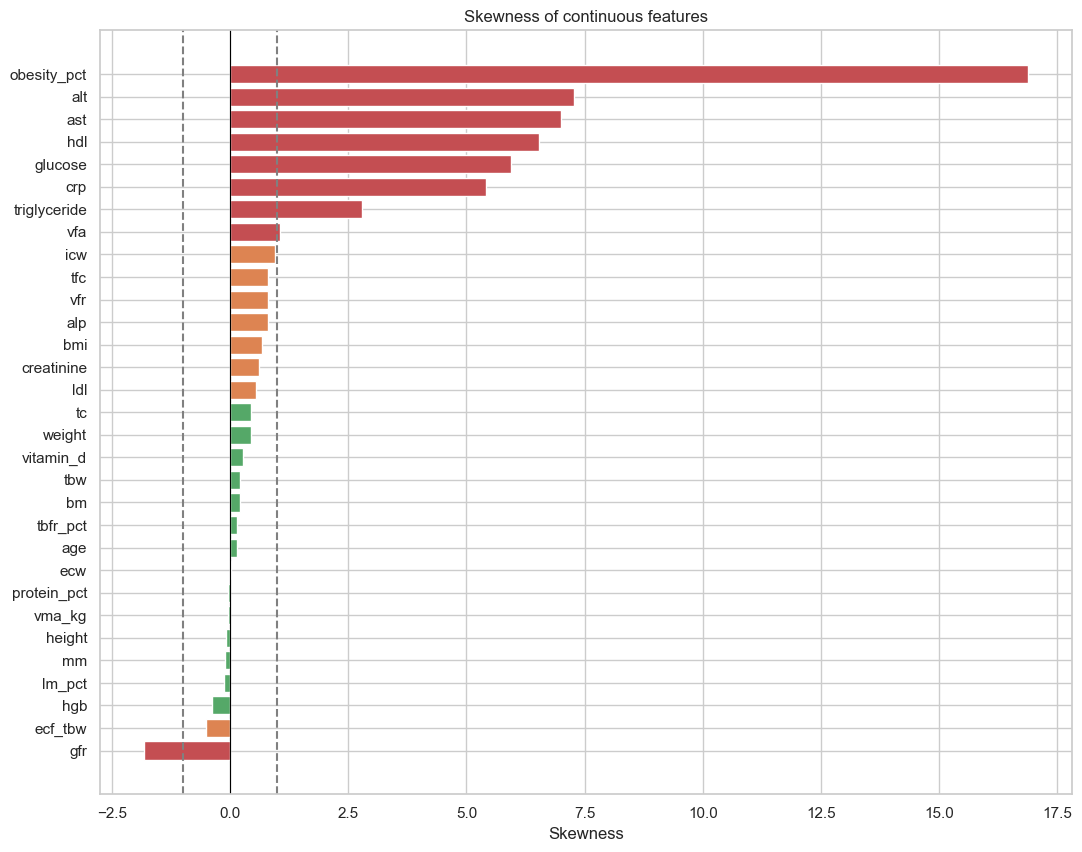
\includegraphics[
        width=0.88\linewidth,
        keepaspectratio
    ]{media/skewness_continous_features.png}
    \caption{Skewness of the continuous variables. The dashed vertical lines
    indicate the threshold of $|\mathrm{skewness}| = 1$ used to identify
    strongly skewed variables.}
    \label{fig:continuous-skewness}
\end{figure}

Figure~\ref{fig:continuous-skewness} shows that several continuous measurements
were strongly right-skewed. The most extreme case was
\texttt{obesity\_pct}, with a skewness of approximately 16.87, followed by
ALT (7.28), AST (6.99), HDL (6.53), glucose (5.94), and CRP (5.41).
Triglyceride was also strongly positively skewed (2.79), while GFR exhibited
substantial negative skewness ($-1.81$). VFA showed a smaller but still notable
positive skewness of approximately 1.06. In contrast, most of the remaining
continuous measurements were relatively close to symmetric.

These results are consistent with the earlier outlier analysis. In particular,
the extreme skewness of \texttt{obesity\_pct} appears to be strongly influenced
by the unusually large observation identified during data-quality assessment.
Similarly, the long right tails observed for ALT, AST, glucose, CRP, and
triglyceride indicate that a small number of participants have measurements
considerably larger than the majority of the sample. These observations were
not removed solely because they increased skewness, since extreme values may
represent clinically plausible measurements.


\subsection{Data Construction}
\label{subsec:data-construction}

The data-construction stage focused on producing a consistent analytical dataset
while preserving the original source data. No additional derived clinical
variables were introduced unless they had a clear analytical justification.

Three logical versions of the dataset were maintained:

\begin{itemize}
    \item \textbf{Raw data:} the original dataset retained without
          modification;

    \item \textbf{Cleaned data:} the dataset after validation of field names,
          data types, categorical values, ranges, duplicates, and potential
          data-quality issues;

    \item \textbf{Model-ready data:} the final analytical dataset containing
          \textit{Gallstone Status} and the predictor variables used by the
          Python modelling pipeline.
\end{itemize}

This separation ensures that preprocessing operations do not overwrite the
source dataset and allows each transformation to be reproduced from the raw
data through the Python scripts.


\subsubsection{Data Partitioning}
Iteration 4 uses five stratified 70\% training / 30\% test holdouts, with seeds 42, 7, 21, 84 and 123. Each split has 223 training and 96 test records. The disease-positive outcome is class 1 (source code 0). Saved source-row membership permits an audit of the disjoint training and test partitions.

Three-fold stratified cross-validation is performed exclusively within the 223 training records. Every inner fit learns its own imputers, 20-feature selector and continuous-variable transformations. The selected hyperparameters are then refitted on the complete training partition and evaluated once on its test partition at the fixed threshold 0.5. Stacking additionally generates training-only out-of-fold base probabilities for its meta-learner. Original numeric ordinal/binary category codes are retained without one-hot expansion.

The five holdouts reuse a cohort and therefore overlap; they measure sensitivity to split choice rather than five independent external validations. Test outcomes are descriptive evaluation evidence and cannot determine tuning settings or a validation-selected model.

\subsection{Data Integration}
\label{subsec:data-integration}

Although the Gallstone dataset was originally obtained as a single public
dataset, an explicit integration exercise was conducted to demonstrate how
logically separate healthcare data sources can be combined into a unified
analytical table.

The original dataset was preserved unchanged and divided into two logical CSV
sources. The first file,
\path{gallstone_demographic_clinical.csv}, contains 319 records and
9 fields describing demographic and clinical characteristics. The second file,
\path{gallstone_biological_body_composition.csv}, contains the same
319 participants and 33 fields describing biological, laboratory, and
body-composition measurements.

A unique \texttt{record\_id}, ranging from 1 to 319, was included in both
tables as the one-to-one integration key. Both tables also contained
\textit{Gallstone Status} so that target consistency could be verified before
integration. However, \textit{Gallstone Status} was not used as a merge key
because it does not uniquely identify an individual participant.

Integration was implemented using the \texttt{pandas.merge()} operation with
\texttt{record\_id} as the matching field. The merge was configured as a
one-to-one operation so that duplicate identifiers or unexpected many-to-one
relationships could be detected explicitly.

Post-integration quality checks verified that all 319 participant records were
retained and that no unmatched identifiers or additional missing values were
introduced by the merge.

The duplicated \textit{Gallstone Status} fields from the two logical data
sources were compared before one copy was removed from the final analytical
table. The \texttt{record\_id} field was retained for traceability and quality
control but excluded from the predictor set used for model development.

This integration exercise represents a simplified version of a realistic
healthcare environment in which demographic and clinical data may be stored
separately from laboratory or body-composition measurements. The Python
workflow demonstrates how these sources can be integrated while maintaining
record integrity and preventing inappropriate use of the target variable as an
integration key.


\subsection{Data Reformatting}
\label{subsec:data-reformatting}

The original Gallstone dataset was provided in Microsoft Excel format
(\texttt{.xlsx}). The file was loaded programmatically using
\texttt{pandas.read\_excel()} and subsequently exported to comma-separated
values (\texttt{.csv}) where appropriate for intermediate storage and
reproducible processing.

CSV was selected as an intermediate format because it provides a simple,
platform-independent representation of tabular data and avoids spreadsheet
formatting that is irrelevant to the modelling process. The use of CSV was not
a modelling requirement, however, because the Python pipeline can also operate
directly on Excel or other structured tabular formats.

During reformatting, variable names were standardised and unnecessary
spreadsheet-specific formatting was removed. The resulting fields were then
classified according to their analytical meaning.

Continuous clinical and body-composition measurements, such as BMI, glucose,
triglyceride, weight, and total body water, were represented as numerical
variables.

Binary variables such as Coronary Artery Disease, Hypothyroidism,
Hyperlipidemia, and Diabetes Mellitus were stored as categorical or binary
indicators rather than being interpreted as continuous measurements.

Variables representing ordered clinical levels were treated as ordinal
variables when their coding reflected an increasing degree of severity or
disease burden.

The target variable, \textit{Gallstone Status}, was represented internally as a
binary label for model training while human-readable labels
(\textit{Gallstone Absent} and \textit{Gallstone Present}) were used in
tables and visualisations.

The final model-ready dataset therefore contained consistent field names,
validated data types, clearly defined variable roles, and a reproducible schema
that could be used directly by the subsequent Python-based feature engineering
and modelling pipeline.


\subsection{Reproducible Open-Source Preparation Pipeline}
\label{subsec:python-preparation-pipeline}

The complete preparation process was implemented as a script-based
open-source workflow. At a high level, the pipeline consisted of:

\begin{enumerate}
    \item loading the source data using \texttt{pandas};
    \item standardising variable names and data types;
    \item validating missing values, duplicates, coding ranges, and
          observations;
    \item performing exploratory outlier and distribution checks;
    \item integrating logically separated datasets using
          \texttt{pandas.merge()};
    \item constructing the final predictor and target datasets;
    \item creating stratified training/test holdouts and training-only CV folds using
          \texttt{scikit-learn};
    \item fitting any required preprocessing operations using the training
          subset only; and
    \item passing the resulting datasets to the machine-learning modelling
          pipeline.
\end{enumerate}

The use of an open-source Python stack provides several advantages for this
project. Each operation is explicitly defined in code, preprocessing decisions
can be version-controlled, experiments can be reproduced using fixed random
seeds, and identical transformations can be consistently applied across
multiple candidate models.

The resulting workflow therefore provides a transparent and reproducible
transition from the original Gallstone dataset to the datasets used for model
training, validation, and final evaluation.

\paragraph{Iteration 4 correction: preserve existing ordinal codes.}
The supplied predictors are already numerically encoded, including ordered codes such as 1, 2, 3, and 4 and binary indicators. These values are retained as provided: no one-hot expansion, category reindexing, or arbitrary replacement numbering is applied. Missing coded values are imputed by the training-partition mode; continuous measurements are median-imputed and scaled within training. The label mapping is separate: source gallstone status 0 remains model class 1 (gallstones present). Numeric category codes must reflect their documented order; storing a nominal category as a number does not itself establish ordinality. For logistic regression, a single ordinal coefficient imposes equal log-odds increments per code step, while trees can learn thresholds between levels. Historical fitted models and scores used the previous representation and do not validate this correction.


\subsection{Data Reduction and Projection}
\label{sec:data-reduction}
\subsubsection{Training-only Feature Selection}
Both candidate selectors retain 20 original source fields. CART importance selection uses a decision tree with maximum depth 5 and minimum leaf size 4, retaining the 20 largest impurity importances. Recursive feature elimination (RFE) uses the same CART estimator, removes one field per step and refits until 20 remain. Imputation precedes selection, and the selected continuous fields are transformed after selection; ordinal category codes remain unchanged.

Both methods are supervised and therefore fitted only on training records. Every inner CV fit repeats imputation and selection, so its validation records cannot influence the retained fields. Stacking maintains a complete preparation pipeline for each base learner and refits selection inside its own out-of-fold construction. After tuning, the final pipeline refits selection using the complete 223-record training partition, before predicting the 96 held-out records.

Selected-feature CSVs include source names, selection flags and ranks, separately for each stacking base learner. Selection may vary across seeds and fits. Impurity importance can favour predictors with more available split points and does not establish a clinical effect. The four controlled preparation benchmarks in Section 8 evaluate selector and transformation changes while maintaining fixed model settings and test membership.


\section{Data-Mining Method Selection}
\label{sec:dm-method-selection}
\subsection{Learning Paradigm and Research Objective}
\label{subsec:matching-dm-methods}

The objective is to estimate gallstone presence from demographic, clinical,
laboratory, and body-composition measurements. All 319 records have a known
binary outcome, making \textbf{supervised learning} the appropriate primary
paradigm: predictions can be compared with observed labels on held-out records.
\textbf{Unsupervised learning} can reveal structure without those labels, but
similarity between patients does not necessarily correspond to disease
status. It therefore supports exploration rather than providing the principal
answer to the research question.

\subsection{Comparison of Data-Mining Methods}
\label{subsec:dm-family-comparison}

The learning paradigm must be narrowed to a method whose output matches the
objective. Table~\ref{tab:dm-family-comparison} distinguishes this decision
from the choice of a particular algorithm.

\begin{table}[H]
\centering
\small
\caption{Suitability of data-mining methods for the gallstone-prediction objective.}
\label{tab:dm-family-comparison}
\begin{tabularx}{\textwidth}{@{}p{2.8cm}XX@{}}
\toprule
Method & Intended output & Suitability for this project \\
\midrule
\textbf{Classification} &
A known class and, where supported, its probability. &
Directly matches labelled gallstone presence/absence and permits evaluation
of discrimination, missed cases, and false alarms. Selected as the primary
method. \\
Continuous-value prediction (regression) &
A numerical quantity, such as a laboratory concentration or severity score. &
The target is a category, not a continuous measurement. This would answer a
different question. Classification is also predictive; the distinction here
concerns the type of output. \\
Segmentation (clustering) &
Groups of observations with similar predictor profiles. &
Useful for exploratory subgroups, but groups need not correspond to
gallstone status. Cluster membership alone is not a validated disease
prediction. \\
Association discovery &
Frequently co-occurring conditions or measurement patterns. &
Useful for hypothesis generation, but support and confidence do not establish
held-out discrimination or an acceptable false-negative rate. Outcome-directed
rules would still require supervised classification evaluation. \\
Anomaly detection &
Observations that differ from a reference pattern. &
Supports review of unusual measurements, but gallstone cases comprise roughly
half the sample and cannot be equated with anomalies. \\
\bottomrule
\end{tabularx}
\end{table}

Dimensionality reduction and feature selection are supporting preparation
methods, not substitutes for predicting the labelled outcome. Likewise,
forecasting future onset or modelling time to diagnosis would require
longitudinal or event-time information not used by the current workflow.
The available evidence supports classification of recorded gallstone status,
not a demonstrated forecast of future disease.

\subsection{Selected Method and Success Criteria}
\label{subsec:dm-method-decision}

The selected method is \textbf{supervised binary classification with
probability estimation}. It provides the required patient-level output and
directly supports the project benchmarks of ROC--AUC at least 0.80 and
gallstone-class sensitivity at least 0.80. Specificity, precision, F1,
stability, and interpretability are needed alongside these measures: predicting
every patient as positive could satisfy sensitivity while producing
unacceptable false alarms.

The source coding is 0 = gallstones present and 1 = absent. The Python
modelling target is recoded to 1 = present and 0 = absent, so
$\mathrm{FNR}=\mathrm{FN}/(\mathrm{FN}+\mathrm{TP})=1-\mathrm{sensitivity}$
measures missed gallstone cases. These are analytical project benchmarks,
not clinical deployment thresholds. The following section compares algorithms
within this chosen method and explains how the implemented models are built
and selected.

\subsection{CRISP-DM Design, Tools and Spark/Colab Execution}
\label{subsec:crispdm-tools}
The latest completed native Spark holdout output retrieved from Google Drive supplies completed evidence for standardization with all thirty-eight predictors, three native model families and five holdouts. Section~\ref{sec:model-building} contains those measured scores and confusion matrices. The primary Colab notebook extends that workflow to CART20, RFE20 and RFE10, allowing the selection-method and feature-count comparisons to be repeated within Spark. Selection and scaling remain inside the training-CV pipeline, and the extension records split membership, selected fields, candidate CV scores and fitted models.

Native Spark CART20, RFE20 and RFE10 are implemented in the new pipeline extension. The submitted evidence currently includes the measured all-field Colab baseline; additional native feature-selection scores will be inserted only after a complete Spark run.


Native Spark scaling divides continuous predictors by their training sample standard deviation without centering, matching the saved Spark baseline. This differs from the centered standardization in the Python comparisons above. Consequently, those comparisons explain the completed preparation experiments but cannot substitute for native Spark results. The new feature-selection runs are prepared for Colab; the report uses the saved Spark evidence until their execution is complete.


The tools implement the CRISP-DM cycle rather than define a new learning objective. Spark SQL and the saved Colab visualizations support data understanding; Spark ML pipelines support preparation and modelling; training-CV traces and held-out predictions support evaluation; GitHub versions source and report artifacts, and Google Drive persists Colab inputs and results. The retained Python/Optuna workflow provides the separately labelled five-family comparison. Reproducible runtime, data/code signatures and checkpointed outputs connect these stages. Platform choice is not evidence of predictive superiority.


\section{Algorithm Selection and Parameterisation}
\label{sec:algorithm-selection}
\subsection{Exploratory Algorithm Analysis within the DM Objectives}
\label{subsec:algorithm-exploration}
The data-mining objective is supervised classification of recorded gallstone presence, with project targets of ROC--AUC at least 0.80 and disease-class recall at least 0.80. Exploration therefore asks whether a candidate learns useful discrimination beyond a no-information baseline, whether additional flexibility is justified on this small cohort, and whether its predictions can support a sensitivity-oriented decision rule. Recall at a fixed threshold also depends on calibration and the false-positive trade-off, so ROC--AUC alone does not establish that both objectives are met. This step combines model-family reasoning with measured \emph{training-only} CV evidence. The held-out evaluation in Section~\ref{sec:model-building} answers the subsequent question of how the selected procedures generalise.

\subsubsection{Statistical-based Family: Logistic Regression}
Logistic regression models a linear combination of predictors on the log-odds scale and converts it to a disease probability. It supplies a regularised, relatively interpretable reference for the demographic, laboratory and body-composition fields. It does not require normally distributed predictors, but its additive linear predictor may miss nonlinear effects and interactions unless these are constructed explicitly. Correlated measurements can affect coefficient stability, motivating training-only selection and regularisation. The standalone model's regularisation strength is tuned; the logistic components inside stacking remain fixed as specified in Section 6.3. Its inclusion tests whether more complex learners improve on a compact statistical model rather than assuming complexity is beneficial.

\subsubsection{Tree-based Families: Bagging and Boosting}
\paragraph{Random forest.} Random forest averages many trees fitted with sampling and predictor randomisation. It can represent nonlinear thresholds and interactions without requiring one additive relationship across the cohort. This is useful for heterogeneous clinical measurements, but the resulting ensemble is less directly interpretable than logistic regression. Tree depth, leaf size and feature sampling must constrain variance when the training set contains only 223 records. Its training-CV performance tests whether interaction flexibility adds useful information beyond the statistical reference.

\paragraph{XGBoost.} XGBoost sequentially adds regularised trees to improve an objective. Learning rate, tree count, depth, row/column sampling and regularisation control the balance between fit and overfitting. This family tests whether controlled boosting captures patterns not recovered by bagging. A high training score alone would be insufficient; the search evaluates each proposed configuration on inner validation folds.

\paragraph{LightGBM.} LightGBM provides a different gradient-boosted-tree implementation and leaf-growth strategy. Its leaf count and minimum child size are important controls for the small cohort. It is included to compare boosting implementations empirically under the same training partitions, not because computational efficiency establishes higher predictive accuracy. The additional flexibility requires training-CV support.

\paragraph{Native Spark GBT.} Spark gradient-boosted trees supply a native Spark boosting candidate alongside Spark logistic regression and random forest. Its estimator and parameter grid differ from XGBoost and LightGBM. Consequently, its evidence is tracked separately rather than treating its scores as interchangeable with either Python boosting library.

\subsubsection{Combined Family: Stacking}
Stacking combines logistic regression, random forest, XGBoost and LightGBM base probabilities through a logistic meta-learner. Its purpose is to test complementary prediction patterns across statistical, bagging and boosting approaches. The meta-learner is trained on out-of-fold base predictions; each base learner's preparation is fitted within that construction. This avoids training the meta-model on predictions obtained by fitting the same observations. Stacking adds computational cost and can propagate unstable base predictions, so it is retained only as an empirically evaluated candidate, not assumed to outperform simpler learners. The completed search jointly tunes the two boosting base learners while leaving the base and meta logistic regressions unchanged.

\subsubsection{Dummy Family: No-information and Chance Baseline}
The dummy establishes what can be achieved without any patient predictors. The implemented \texttt{DummyClassifier} with \texttt{strategy='prior'} learns the training class proportions and assigns the same disease probability to every patient. Its constant probability has ROC--AUC 0.50 and therefore supplies a chance-discrimination reference. This is the relevant baseline for a comparison with random/no-information choices, but it is \emph{not} a randomly sampled classifier: a uniform or stratified random-label strategy would be a separate experiment. At threshold 0.5 the prior baseline can predict every record as positive, yielding perfect recall and zero specificity. It must therefore be assessed alongside discrimination and false positives rather than praised for recall alone. The distinction follows the \href{https://scikit-learn.org/stable/modules/generated/sklearn.dummy.DummyClassifier.html}{documented dummy strategies}.

\subsubsection{Empirical Training-CV Exploration and Selection}
The five predictive families and dummy receive matched training partitions and stratified three-fold CV memberships. The fixed comparison uses the predeclared RFE20/standardization preparation; the tuned comparison gives each predictive family twenty Optuna trials per seed. Every inner fit repeats imputation, RFE and scaling, including base pipelines within stacking. The following table is the empirical evidence used in Step 6.1, rather than a conceptual comparison postponed to the result section.

\begin{table}[H]
\centering\small
\caption{Algorithm exploration: training-only three-fold CV AUC, mean and sample SD across five seeds.}
\label{tab:holdout-selection}
\begin{tabular}{lrr}
\toprule
Model & Fixed CV AUC & Best-trial CV AUC \\
\midrule
Logistic regression & 0.809 $\pm$ 0.019 & 0.819 $\pm$ 0.025 \\
Random forest & 0.842 $\pm$ 0.021 & 0.852 $\pm$ 0.015 \\
XGBoost & 0.838 $\pm$ 0.016 & 0.854 $\pm$ 0.021 \\
LightGBM & 0.832 $\pm$ 0.024 & 0.848 $\pm$ 0.021 \\
Stacking & \textbf{0.845} $\pm$ 0.017 & \textbf{0.855} $\pm$ 0.015 \\
Prior dummy & 0.500 $\pm$ 0.000 & Not tuned \\
\bottomrule
\end{tabular}
\end{table}
Training-CV choices are seed 7: XGBoost (0.888), seed 21: Random forest (0.840), seed 42: Stacking (0.862), seed 84: Random forest (0.857), seed 123: Stacking (0.852). These are best-trial training scores, not test scores.


All predictive families exceed the dummy's mean CV AUC of 0.500. Fixed stacking has the highest mean (0.845), narrowly followed by random forest (0.842) and XGBoost (0.838); logistic regression has the lowest predictive-family mean (0.809). The best-trial means increase to 0.855 for stacking, 0.854 for XGBoost, 0.852 for random forest, 0.848 for LightGBM and 0.819 for logistic regression. The search improves the observed training-CV objective by approximately 0.010--0.016, but the best-trial score is optimistic after selecting among trials and is not an unbiased test-performance estimate.

These findings justify retaining nonlinear families alongside the statistical reference. They do not justify a universal winner: the gap between the three leading tuned means is only 0.003, and the seed-specific CV choices are random forest twice, stacking twice and XGBoost once. All five families are consequently retained in the planned held-out benchmark, while any seed-specific family selection uses its training-CV ranking. Logistic regression remains useful as the interpretable reference, and the dummy establishes the minimum discrimination standard. High CV AUC does not establish the recall target at threshold 0.5; that trade-off is evaluated on the held-out records. No test result is used retrospectively to choose the family, preparation or Optuna objective.

\subsubsection{Why Cross-validation Represents the Selection Scenario}
In practical model development, candidate models are fitted on training observations, compared on validation observations, and then evaluated on records excluded from those decisions. The inner folds mimic repeated validation opportunities within the available training sample. They reduce dependence on one small validation allocation and allow every outer-training record to contribute to validation once per three-fold cycle. Three folds are a computational compromise for repeated RFE, stacking and tuning; they do not make validation uncertainty disappear.

For each Iteration 4 seed, the 223-record outer training set supplies three inner folds (approximately 148--149 fit records and 74--75 validation records). Mean validation AUC selects parameters and, where applicable, the candidate family. The selected pipeline is refitted on all 223 training records before the locked procedure predicts the 96 outer test records. The test set is an assessment set, not another tuning fold. Repeatedly choosing settings from its scores would invalidate this separation. The same rule covers preprocessing, feature count, threshold or calibration choices. This design follows the distinction between tuning and outer evaluation in the \href{https://scikit-learn.org/stable/modules/cross_validation.html}{cross-validation guidance}.

This mimics selecting a procedure before observing new patient outcomes from the same source population. It does not reproduce temporal deployment, a new hospital or external clinical validation. The five outer holdouts overlap, and stratification preserves class representation rather than supplying independent cohorts. Section 7 therefore reports held-out outcomes separately from the development evidence in this subsection.

\subsubsection{Training-CV Exploration and Selection in Native Spark}
The Spark comparison retains the same linear/bagging/boosting rationale, using native logistic regression, random forest and GBT. Its completed baseline retains all thirty-eight predictors and uses three-fold training-only ROC--AUC to choose a configuration within each family. These model grids are a separate comparison from the five-family Python/Optuna study. The saved Spark notebook confirms \texttt{tune=True}, but its retained metrics contain test outcomes only: numerical inner-CV AUC values and the complete winning-parameter trace are unavailable in that baseline snapshot. Table~\ref{tab:spark-cv-exploration} records the selection procedure and evidence status without substituting test scores for missing validation scores.

\begin{table}[H]
\centering\small
\caption{Native Spark training-CV exploration and model-selection evidence. Numerical CV scores are not retained in the completed baseline.}
\label{tab:spark-cv-exploration}
\begin{tabularx}{\textwidth}{@{}p{2.7cm}p{1.5cm}XX@{}}
\toprule
Candidate & Settings & Validation selection rule & Available evidence \\
\midrule
Logistic regression & 3 & Maximum mean three-fold training AUC within family. & Tuned execution confirmed; inner-CV AUC not retained. \\
Random forest & 4 & Same folds and AUC objective; compare depth and tree count. & Tuned execution confirmed; inner-CV AUC not retained. \\
Spark GBT & 4 & Same folds and AUC objective; compare depth and learning step. & Tuned execution confirmed; inner-CV AUC not retained. \\
\bottomrule
\end{tabularx}
\end{table}

No empirical cross-family Spark winner is claimed from missing CV scores. All three families are retained for the planned Spark holdout comparison, whose test metrics appear in Section 7. The updated holdout scripts print every candidate CV AUC and selected parameter set, and save \path{training_cv_results.csv}, \path{training_cv_summary.csv} and per-model \path{cv_search.json}. These training-only traces and selected-field artifacts allow the next completed run to supply a numerical Spark exploration table; the historical test-only output is not retroactively assigned CV scores. This evidence gap is specific to the saved native baseline and does not remove the measured five-family CV comparison above. The optional CUDA XGBoost research extension is a hybrid Spark-preparation/driver-GPU implementation, not an additional completed native Spark baseline.

\subsection{Controlled Preparation and Candidate Settings}
The native Spark extension implements all-field standardization, CART20, RFE20 and RFE10 as matched preparation versions. Its persistable selector uses native Spark CART importance and one-field-at-a-time RFE. All supervised selection and scaling are refitted within CV. The separate completed Python RFE10 iteration tests the feature-count change against its fixed RFE20 benchmark.
CART importance and CART-based recursive feature elimination (RFE) each retain 20 original fields. Both are tested with Yeo--Johnson followed by standardization, and with standardization alone. Ordinal category codes pass through unchanged. These four fixed-parameter benchmarks isolate selector and transformation changes; the predeclared RFE/standardization configuration is used for the tuning comparison, without selecting it from test results.

\subsection{Training-only Optuna Parameter Search}
Each model receives 20 Optuna TPE trials for each of five seeds, scored by mean three-fold training ROC--AUC. Standalone logistic regression searches $C\in[0.01,100]$ on a logarithmic scale. Random forest searches tree count 40--160 in steps of 20, maximum depth 2--8, minimum leaf size 2--10 and maximum feature fraction (square root, 0.5, 1.0). XGBoost searches tree count 40--160, learning rate 0.01--0.15 (log), depth 1--4, row and column sampling 0.6--1.0, and L2 regularisation 0.1--10 (log). LightGBM searches tree count 40--160, learning rate 0.01--0.15 (log), leaves 3--15, minimum child records 10--40, column sampling 0.6--1.0 and L2 regularisation 0.1--10 (log).

Stacking searches the twelve settings of its layer-1 XGBoost and LightGBM pipelines jointly. Its base logistic regression and meta logistic regression remain fixed at $C=1$; its forest and three-fold stacking configuration remain fixed. RFE retains 20 fields with step 1 and a CART selector of depth 5 and minimum leaf size 4. These selector controls are compared through the controlled preprocessing benchmarks rather than included in the classifier search. The fixed search budget is reproducible but cannot establish exhaustive optimisation. Per-model trial CSVs, best-parameter JSONs and fitted pipelines document all tested values, including unsuccessful improvement attempts.

\subsection{Native Spark Tuning and Parameterisation}
\label{subsec:native-spark-tuning}
The completed native baseline and the preparation extension use the same classifier grids in Table~\ref{tab:spark-tuning-grid}. Spark stratified three-fold training CV maximizes ROC--AUC independently for each family and outer seed. The best configuration is refitted on the outer training partition; held-out scores never choose a grid setting. Fixed estimator controls are listed separately from searched values so the table does not imply that they were empirically optimised.

\begin{table}[H]
\centering\small
\caption{Native Spark classifier tuning grids and fixed controls; three-fold training-only CV is used for every grid.}
\label{tab:spark-tuning-grid}
\begin{tabularx}{\textwidth}{@{}p{2.5cm}XXp{1cm}@{}}
\toprule
Model & Searched parameters and values & Fixed estimator controls & Grid size \\
\midrule
Logistic regression & \texttt{regParam}: 0.001, 0.01, 0.1. & \texttt{elasticNetParam}=0; \texttt{maxIter}=300. & 3 \\
Random forest & \texttt{maxDepth}: 3, 5; \texttt{numTrees}: 40, 60. & \texttt{minInstancesPerNode}=4; seed fixed per run. & 4 \\
Spark GBT & \texttt{maxDepth}: 2, 3; \texttt{stepSize}: 0.05, 0.1. & \texttt{maxIter}=60; \texttt{minInstancesPerNode}=4; seed fixed per run. & 4 \\
\bottomrule
\end{tabularx}
\end{table}

Across the three families, these grids require 33 inner classifier fits and three outer-training refits per seed, excluding preprocessing costs. The completed baseline retains all thirty-eight fields. The extension compares all fields, CART20, RFE20 and RFE10 with native CART depth five and minimum four instances per node; those selector settings are fixed rather than classifier-grid dimensions. Every selector is fitted inside training CV. The newer LOPO implementation reuses a prepared inner partition across classifier settings when preparation parameters are unchanged, preserving this separation while reducing repeated work.

The original baseline saves fitted best pipelines and test metrics but not all candidate CV scores. The extension writes those scores to \path{cv_search.json}; their future availability is not treated as retrospective evidence that every setting in this table improved performance. The CUDA XGBoost Optuna search belongs to the separate research LOPO workflow and is not part of this native Spark holdout grid.


\section{Model Execution and Statistical Results}
\label{sec:model-building}
\subsection{Non-Spark Holdout Results: Five Optuna-tuned Models}
\label{subsec:python-optuna-execution}
The completed non-Spark experiment evaluates \textbf{logistic regression, random forest, XGBoost, LightGBM and stacking}. Each uses the same five stratified 70/30 holdouts (seeds 42, 7, 21, 84 and 123), with 223 training and 96 test records per split. RFE retains twenty source fields, continuous predictors receive standardization, and ordinal category codes remain unchanged. Each family receives twenty Optuna trials per seed, evaluated by three-fold training-only ROC--AUC. The selected configuration is refitted on the 223 training records and then predicts the untouched 96-record test partition. No held-out record enters fitting, RFE, scaling or parameter selection. The search spaces and training-CV evidence are documented in Section~\ref{sec:algorithm-selection}.

\begin{table}[H]
\centering\small
\caption{Completed non-Spark Optuna-tuned holdout results: mean and sample SD across five matched seeds, RFE20 and standardization. Highest displayed means are bold.}
\label{tab:holdout-optuna-test}
\begin{tabular}{lrrrrr}
\toprule
Model & AUC & Accuracy & Precision & Recall & F1 \\
\midrule
Logistic regression & \textbf{0.843} $\pm$ 0.037 & 0.754 $\pm$ 0.041 & 0.732 $\pm$ 0.046 & 0.808 $\pm$ 0.071 & 0.766 $\pm$ 0.040 \\
Random forest & 0.803 $\pm$ 0.032 & 0.731 $\pm$ 0.027 & 0.704 $\pm$ 0.034 & 0.804 $\pm$ 0.043 & 0.750 $\pm$ 0.022 \\
XGBoost & 0.793 $\pm$ 0.033 & 0.746 $\pm$ 0.032 & 0.713 $\pm$ 0.027 & \textbf{0.825} $\pm$ 0.062 & 0.764 $\pm$ 0.034 \\
LightGBM & 0.793 $\pm$ 0.015 & 0.723 $\pm$ 0.030 & 0.701 $\pm$ 0.021 & 0.779 $\pm$ 0.079 & 0.736 $\pm$ 0.040 \\
Stacking & 0.824 $\pm$ 0.038 & \textbf{0.762} $\pm$ 0.039 & \textbf{0.740} $\pm$ 0.044 & 0.812 $\pm$ 0.042 & \textbf{0.774} $\pm$ 0.034 \\
\bottomrule
\end{tabular}
\end{table}


Table~\ref{tab:holdout-optuna-test} contains \textbf{test results}, not the training-CV scores shown in Section 6.1. It summarises twenty-five completed tuned model/seed evaluations from \path{results/holdout/metrics_per_seed.csv}, with fitted pipelines, predictions, best parameters and trial traces retained per model. Mean and sample standard deviation describe the five split-specific outcomes. The partitions overlap, so this variation is not independent cohort replication. Metrics use gallstones-present class 1 and a probability threshold of 0.5.

Among the five Optuna-tuned candidates, logistic regression has the highest mean test AUC (0.843). Stacking has the highest mean accuracy (0.762), while XGBoost has the highest mean recall (0.825). These are metric-specific observations rather than an overall ranking: discrimination, false negatives and false positives need to be considered together. Both project targets (AUC $\geq0.80$ and recall $\geq0.80$) were met in two of five splits for logistic regression, random forest and LightGBM, and three of five for XGBoost and stacking. Training-CV selection and observed test performance can therefore favour different families without contradicting the evaluation procedure.

\begin{figure}[H]
\centering
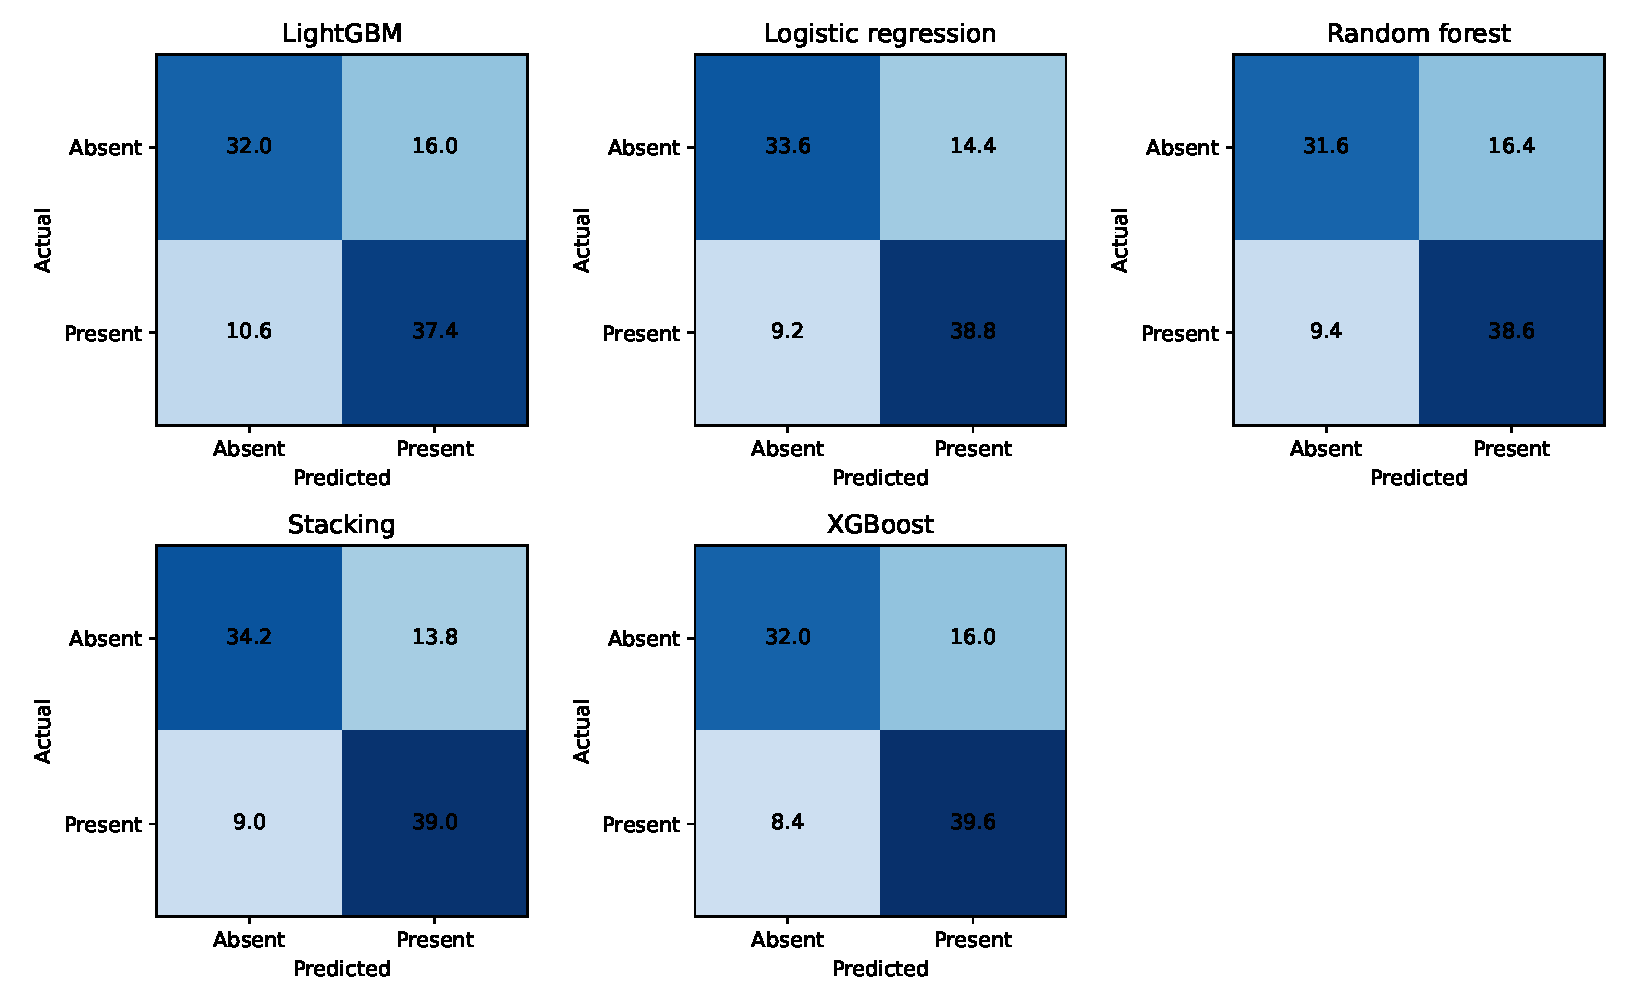
\includegraphics[width=.85\textwidth]{figures/modeling/holdout_average_cm.pdf}
\caption{Average non-Spark test confusion counts across five holdouts for each Optuna-tuned family. Fractional counts arise from averaging 96-record test sets.}
\end{figure}

\subsection{Non-Spark Fixed-parameter Holdout Reference}
The following fixed-model reference uses the same RFE20 preparation and test memberships. It supports comparison with the tuned procedure without mixing fixed and tuned rows in the main Optuna result table. The training-prior dummy is included as a baseline; its perfect recall is obtained by predicting every record as positive and is accompanied by zero specificity.

\begin{table}[H]
\centering\small
\caption{Non-Spark fixed-parameter holdout reference: RFE20 and standardization with the same five test partitions. Highest displayed means are bold, including ties and the prior dummy.}
\label{tab:holdout-fixed-test}
\begin{tabular}{lrrrr}
\toprule
Model & AUC & Recall & Specificity & Accuracy \\
\midrule
Logistic regression & \textbf{0.832} $\pm$ 0.042 & 0.817 $\pm$ 0.063 & 0.688 $\pm$ 0.081 & \textbf{0.752} $\pm$ 0.046 \\
Random forest & 0.808 $\pm$ 0.047 & 0.783 $\pm$ 0.041 & 0.700 $\pm$ 0.075 & 0.742 $\pm$ 0.041 \\
XGBoost & 0.801 $\pm$ 0.030 & 0.796 $\pm$ 0.073 & 0.688 $\pm$ 0.042 & 0.742 $\pm$ 0.032 \\
LightGBM & 0.799 $\pm$ 0.027 & 0.775 $\pm$ 0.063 & 0.679 $\pm$ 0.035 & 0.727 $\pm$ 0.028 \\
Stacking & 0.824 $\pm$ 0.029 & 0.787 $\pm$ 0.048 & \textbf{0.708} $\pm$ 0.074 & 0.748 $\pm$ 0.017 \\
Prior dummy & 0.500 $\pm$ 0.000 & \textbf{1.000} $\pm$ 0.000 & 0.000 $\pm$ 0.000 & 0.500 $\pm$ 0.000 \\
\bottomrule
\end{tabular}
\end{table}


The controlled scaling, selector and feature-count comparisons are interpreted in Section~\ref{sec:multiple-iteration}. The full saved outputs additionally contain specificity, balanced accuracy, false-negative rate, log loss, fit/prediction time and other metrics. A larger search is not assumed to improve every model; its effect is judged against the matched fixed reference.

\subsection{Native Spark Holdout Results in Google Colab}
The native Spark execution provides a separate platform-based holdout evaluation using PySpark for loading, preparation, model fitting, training-only cross-validation, predictions and metrics. The latest completed Colab holdout output retrieved from the shared Google Drive folder trained native Spark logistic regression, random forest and gradient-boosted trees on five stratified 70/30 holdouts (seeds 42, 7, 21, 84 and 123). Each split used 223 training and 96 test records. All 38 source fields were retained; continuous fields were standardized and original ordinal codes were preserved. Three-fold Spark CrossValidator operated on training records only.

\begin{table}[H]
\centering\small
\caption{Completed native PySpark holdout results from Google Drive: mean and sample SD across five seeds. Highest displayed metric means and lowest error rate are bold; ties share highlighting.}
\label{tab:spark-colab-execution}
\resizebox{\textwidth}{!}{\begin{tabular}{lrrrrrrr}
\toprule
Model & AUC & Accuracy & Precision & Recall & Specificity & F1 & Error rate \\
\midrule
Spark GBT & 0.804 $\pm$ 0.045 & 0.721 $\pm$ 0.056 & 0.701 $\pm$ 0.057 & 0.779 $\pm$ 0.043 & 0.662 $\pm$ 0.092 & 0.737 $\pm$ 0.044 & 0.279 $\pm$ 0.056 \\
Logistic regression & \textbf{0.873} $\pm$ 0.027 & \textbf{0.810} $\pm$ 0.029 & \textbf{0.766} $\pm$ 0.042 & \textbf{0.900} $\pm$ 0.040 & \textbf{0.721} $\pm$ 0.072 & \textbf{0.826} $\pm$ 0.023 & \textbf{0.190} $\pm$ 0.029 \\
Random forest & 0.806 $\pm$ 0.056 & 0.715 $\pm$ 0.052 & 0.714 $\pm$ 0.044 & 0.713 $\pm$ 0.081 & 0.717 $\pm$ 0.041 & 0.713 $\pm$ 0.060 & 0.285 $\pm$ 0.052 \\
\bottomrule
\end{tabular}}
\end{table}
All metrics describe the same three models and five 96-record test holdouts, using the full-precision completed Drive output dated 12 October 2026. Recall is sensitivity; error rate equals one minus accuracy. Precision and F1 measure different properties, so their values need not equal accuracy or AUC. These test metrics are separate from training-CV selection evidence.


Table~\ref{tab:spark-colab-execution} consolidates all Spark test metrics from one experiment. The raw output was saved on 12 October 2026 and contains fifteen complete model/seed evaluations. Its full-precision metric file, source notebook invocation and provenance are retained in \path{results/spark_holdout_drive}. Bold entries identify the highest displayed means within each metric column, with ties highlighted together; error rate is minimized. Standard deviations are reported rather than ranked.

The saved execution demonstrates actual use of Spark and Colab, while the GitHub repository supplies the source and saved notebook evidence. It does not establish that the newer CART20/RFE20/RFE10 extension has already run. Its pipeline performs selection within native Spark fits and records the corresponding tuning traces when executed. Spark GBT is a separate implementation from XGBoost and LightGBM.

\begin{figure}[H]
\centering
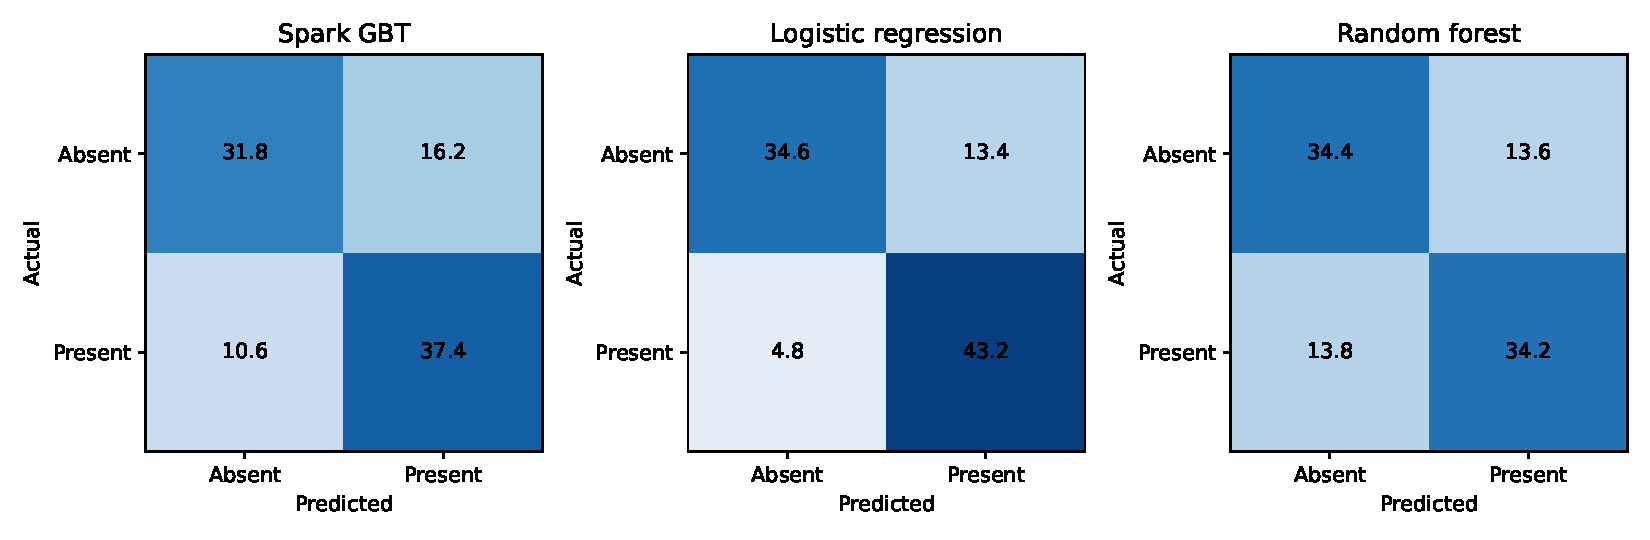
\includegraphics[width=.95\textwidth]{figures/modeling/spark_average_cm.pdf}
\caption{Mean native Spark test confusion counts over the latest five completed Google Drive holdouts. Counts are averaged rather than pooled into an independent new cohort.}
\end{figure}


The native Spark results use all thirty-eight predictors and Spark estimators, whereas the non-Spark Optuna results above use RFE20 and their Python estimator implementations. They demonstrate the two completed workflows; a numerical difference between them cannot be attributed to Spark alone. No LOPO scores are included in these holdout tables.


\section{Interpretation, Evaluation and CRISP-DM Iteration}
\label{sec:multiple-iteration}
\subsection{Controlled Iteration Design}
The iterations examine three preparation decisions: the scaling method, the feature-selection method and the number of selected features. Each comparison changes one decision while keeping the classifier settings, five holdout seeds (42, 7, 21, 84 and 123), 70/30 stratified split and decision threshold of 0.5 unchanged. Imputation, selection and scaling are fitted within the training pipeline, including each training-only cross-validation fold. The held-out records are used for evaluation only. The completed comparisons below use the retained Python workflow; the native Spark execution status is documented separately so that results from the two implementations are not conflated. A fourth iteration changes the assessment strategy to nested LOPO with three-fold training CV, using the observed completed Research Paper outputs in Section~\ref{subsec:validation-strategy-iteration}.

\subsection{Iteration 1: Change in Scaling Method}
The initial configuration applies a Yeo--Johnson transformation followed by standardization to continuous predictors. Yeo--Johnson is intended to reduce distributional skewness, while standardization puts continuous variables on a common scale. The revised configuration removes the power transformation and uses standardization alone, $z=(x-\mu_{\mathrm{train}})/s_{\mathrm{train}}$. This tests whether the additional distributional transformation contributes useful predictive information or whether the simpler scaling procedure is sufficient. Existing ordinal category codes are passed through without one-hot encoding or continuous-variable scaling.

To isolate the scaling effect, CART selection retains twenty fields in both configurations (Iterations A and B). A second matched comparison repeats the scaling change with RFE retaining twenty fields (Iterations C and D). The same five predictive families are evaluated in each configuration, rather than choosing a scaling method from a single model's result.

\begin{table}[H]
\centering\small
\caption{Controlled fixed-model preparation comparisons: mean test AUC over five matched seeds.}
\label{tab:holdout-preparation}
\begin{tabular}{lrrrr}
\toprule
Model & CART+YJ & CART+Std & RFE+YJ & RFE+Std \\
\midrule
Logistic regression & \textbf{0.861} & 0.836 & \textbf{0.864} & \textbf{0.832} \\
Random forest & 0.810 & 0.811 & 0.808 & 0.808 \\
XGBoost & 0.809 & 0.809 & 0.801 & 0.801 \\
LightGBM & 0.805 & 0.814 & 0.794 & 0.799 \\
Stacking & 0.845 & \textbf{0.839} & 0.837 & 0.824 \\
\bottomrule
\end{tabular}
\end{table}


With CART20, changing from Yeo--Johnson plus standardization to standardization alone changes mean test AUC from 0.861 to 0.836 for logistic regression and from 0.845 to 0.839 for stacking. Random forest and XGBoost change little, while LightGBM increases from 0.805 to 0.814. With RFE20, the corresponding logistic regression and stacking AUCs decrease from 0.864 to 0.832 and from 0.837 to 0.824. These results show that the effect depends on the model; standardization alone does not uniformly improve discrimination. It is retained as the common setting for subsequent selector and feature-count comparisons, and it aligns with the available native Spark baseline. This is a controlled experimental choice, not a claim that it is the best scaler for every family.

\subsection{Iteration 2: Change in Feature-selection Method}
The next change replaces a single CART importance ranking with recursive feature elimination (RFE), while retaining twenty source fields. CART selects the twenty highest-importance predictors from one fitted decision tree. RFE repeatedly fits the decision-tree estimator, removes the least-important remaining predictor and refits until twenty predictors remain. Refitting allows rankings to change after a predictor is removed, but requires more fitting work. Both prototype selectors use the same tree controls (maximum depth five and minimum leaf size four) and operate after training-only imputation. RFE therefore changes the selection procedure, rather than introducing a different ranking estimator.

The principal matched comparison is CART20 plus standardization (Iteration B) versus RFE20 plus standardization (Iteration D). The Yeo--Johnson configurations (A versus C) provide an additional check under the other scaling setting. In the standardization comparison, mean AUC changes from 0.836 to 0.832 for logistic regression, 0.811 to 0.808 for random forest, 0.809 to 0.801 for XGBoost, 0.814 to 0.799 for LightGBM and 0.839 to 0.824 for stacking. RFE20 consequently does not outperform CART20 on mean AUC in this configuration. Under Yeo--Johnson, logistic regression increases slightly from 0.861 to 0.864, while the other families decrease. RFE is retained for the following dimensionality experiment to test the effect of reducing its selected subset; its use is not justified by an unsupported claim of universal superiority.

\subsection{Iteration 3: Change in Number of Selected Features}
The final preparation change reduces the RFE subset from twenty to ten source fields (Iteration D versus Iteration F). Standardization, the decision-tree ranking estimator, fixed classifier parameters and all five holdout memberships remain unchanged. This comparison asks whether a smaller input set preserves predictive performance while reducing the number of required fields. It compares fixed models on both sides, so the feature-count effect is not mixed with the separate Optuna tuning experiment. In stacking, selection is fitted separately inside each base learner's training pipeline; saved artifacts confirm ten retained fields for every base learner in the new run.

\begin{table}[H]
\centering\small
\caption{Completed Python prototype feature-count iteration: fixed settings and matched five-seed holdouts, RFE10 minus RFE20. Both use standardization.}
\label{tab:rfe-feature-count}
\begin{tabular}{lrrrr}
\toprule
Model & RFE20 AUC & RFE10 AUC & $\Delta$ AUC & $\Delta$ sensitivity \\
\midrule
LightGBM & 0.799 $\pm$ 0.027 & 0.804 $\pm$ 0.023 & \textbf{+0.005} & \textbf{+0.000} \\
Logistic regression & \textbf{0.832} $\pm$ 0.042 & 0.807 $\pm$ 0.069 & -0.026 & -0.017 \\
Random forest & 0.808 $\pm$ 0.047 & 0.812 $\pm$ 0.047 & +0.004 & -0.004 \\
Stacking & 0.824 $\pm$ 0.029 & \textbf{0.819} $\pm$ 0.047 & -0.006 & \textbf{+0.000} \\
XGBoost & 0.801 $\pm$ 0.030 & 0.802 $\pm$ 0.038 & +0.001 & \textbf{+0.000} \\
\bottomrule
\end{tabular}
\end{table}
This is a controlled feature-count comparison within the Python implementation. It does not supply native Spark CART/RFE scores. All saved selectors and stacking base pipelines retain exactly ten fields in the new run.


The ten-field configuration produces small mean AUC increases for LightGBM, random forest and XGBoost (approximately 0.005, 0.004 and 0.001). Logistic regression decreases by approximately 0.026 and stacking by 0.006. Sensitivity is unchanged for LightGBM, XGBoost and stacking, but decreases by approximately 0.017 for logistic regression and 0.004 for random forest. Thus, reducing the input count has a model-dependent cost. The small positive AUC differences are descriptive results from five matched holdouts, not evidence of statistical superiority. Both feature counts remain documented rather than selecting ten fields solely because the representation is smaller.

\subsection{Iteration 4: Nested LOPO with Three-fold Training CV}
\label{subsec:validation-strategy-iteration}
This iteration changes the evaluation strategy while preserving the distinction between development and assessment. The reported Iteration 4 results use five stratified 70/30 holdouts with three-fold CV inside the training portion. The earlier 70/15/15 design and LOPO discussion retained from Iteration 3 in Part 4 provide historical context; they are not the split membership used for the current 223/96 holdout result tables. A fixed validation split is easy to interpret, but it allocates fewer records to fitting and makes model choice sensitive to a single small validation set. The repeated-holdout/inner-CV design instead uses the training sample more efficiently while keeping an outer test partition.

\begin{table}[H]
\centering\small
\caption{Validation-strategy iteration: historical design, current completed evaluation and separate research extension.}
\label{tab:validation-strategy-iteration}
\begin{tabularx}{\textwidth}{@{}p{2.6cm}XX@{}}
\toprule
Strategy & Development and assessment roles & Evidence/status \\
\midrule
Fixed 70/15/15 & Training fits the model; a validation partition selects settings; a separate test partition assesses the choice. & Historical Iteration 3 design retained in Part 4; not the current holdout results. \\
Five 70/30 holdouts with inner CV & Each 223-record training set supplies three-fold validation; refit on 223 and test on 96. & Completed current non-Spark and native Spark evidence in Section 7. \\
Nested LOPO with three-fold CV & Exclude one patient; tune on the remaining 318 records with three-fold training CV, then refit and predict the excluded patient. & Completed non-Spark Optuna evidence is reported below; the newer Spark/CUDA workflow remains a separate execution. \\
\bottomrule
\end{tabularx}
\end{table}

\subsubsection{Why Test Leave-One-Patient-Out?}
LOPO is the project name for leave-one-out CV when one record represents one patient. With 319 records, the outer loop has 319 held-out predictions per candidate and seed. Each model can use 318 records for fitting, which tests a different training-size and patient-exclusion scenario from the 223-record holdout training sets. This can reveal sensitivity to individual observations while retaining nearly all observations for training, at a substantial fitting cost. It is not evidence that a model generalises to a new hospital or time period. If repeated observations per patient become available, the split must exclude every record from that patient as a group.

\subsubsection{Observed LOPO Results with Three-fold Training CV}
The Research Paper archive contains completed non-Spark nested Optuna runs for logistic regression, random forest, XGBoost, LightGBM and stacking. Each uses seed 42, twenty Optuna trials per outer patient exclusion, and three-fold validation within the remaining 318 records. An inner split fits on 212 records and validates on 106; Optuna selects settings from the three validation AUCs, then the selected pipeline refits on all 318 records before predicting the excluded patient. Every patient is assessed once, giving 319 held-out predictions per model and 1,595 predictions across the five families. The result table therefore evaluates the complete 319-patient cohort, not one patient: 318 is the training-set size of each outer fit, not the number of test patients or the number of outer folds. The imported complete flags, fold checkpoints and all 31,900 completed trial rows were checked; pooled metrics were independently recomputed from the saved probabilities. The method and evidence are copied into \path{iteration4_BDAS/LOPO} without rerunning training.

\begin{table}[H]
\centering\small
\caption{Observed Research Paper results: nested Optuna LOPO with three-fold training CV, seed 42. Scores pool all 319 held-out patients; each outer model trains on 318 records. Highest displayed scores are bold. No bootstrap estimates are included.}
\label{tab:research-optuna-lopo}
\resizebox{\textwidth}{!}{\begin{tabular}{lrrrrrr}
\toprule
Model & AUC & Accuracy & Precision & Recall & Specificity & F1 \\
\midrule
Logistic regression & \textbf{0.868} & \textbf{0.787} & 0.769 & \textbf{0.826} & 0.747 & \textbf{0.796} \\
Random forest & 0.842 & 0.774 & 0.760 & 0.807 & 0.741 & 0.783 \\
XGBoost & 0.851 & 0.784 & 0.764 & \textbf{0.826} & 0.741 & 0.794 \\
LightGBM & 0.840 & \textbf{0.787} & \textbf{0.775} & 0.814 & \textbf{0.759} & 0.794 \\
Stacking & 0.862 & 0.784 & 0.774 & 0.807 & \textbf{0.759} & 0.790 \\
\bottomrule
\end{tabular}}
\end{table}


The table copies the observed \path{metrics.csv} values from the five completed Research Paper runs. Each value is checked against its saved held-out probabilities and original configuration. The final test metrics pool all 319 excluded-patient predictions; they are not training scores on the 318 records, one-patient metrics or three-fold CV tuning scores. Three-fold CV is used only inside each outer training set to select hyperparameters. No bootstrap resampling, additional fitting or newly estimated scores are included in this evidence.

Only seed 42 has a complete archived run for each family. An across-seed mean or variance cannot be measured from this single run, and neither is fabricated. The table reports the original pooled AUC, accuracy, precision, recall, specificity and F1 exactly as observed, rounded for display. Additional independently executed seeds would be needed to report variation across complete repeated runs.

For these observed results, logistic regression has the highest AUC (0.868), followed by stacking (0.862). Logistic regression and LightGBM tie on accuracy (0.787), LightGBM has the highest precision (0.775), and logistic regression and XGBoost tie on recall (0.826). All five meet the AUC and recall benchmarks of 0.80 in this single complete LOPO evaluation. The different metric leaders reinforce the need to assess discrimination, missed cases and false positives together rather than declaring an unconditional winner.

The copied preprocessing uses training-only median/mode imputation, CART-based RFE selecting twenty \emph{source} fields, Yeo--Johnson followed by standardization for continuous fields, and one-hot encoding of selected categorical fields. These are the historical Research Paper settings; they differ from the ordinal-preserving, standardization-only holdout workflow. The saved stacking search also tunes only the logistic meta-learner's $C$, leaving the base learners fixed, whereas the current holdout stacking search tunes the boosting base learners. These differences are preserved to match the measured output. The LOPO scores therefore do not isolate an effect of changing validation strategy: training size, encoding, transformation and some tuning choices also differ. They do not establish a native Spark or GPU result.

The \path{LOPO} folder retains the original three modelling modules, raw input, requirements, tests and per-model configurations, predictions, trial traces and complete flags. \path{LOPO/results/metrics_combined.csv} copies the observed pooled metrics; \path{LOPO/report_results.py} verifies the saved outputs and regenerates the result table; \path{LOPO/provenance.json} records source/output hashes and validation. The original Research Paper folder remains unchanged. New experiments use a separate output directory so this completed evidence snapshot remains identifiable.

\subsubsection{Training, Tuning and Reporting Rules}
Each outer patient's features and outcome are excluded from fitting, preprocessing and parameter selection. Within the remaining records, stratified CV chooses hyperparameters; selection and scaling are refitted inside each inner training fold. The selected procedure is then refitted on the outer training set and predicts the held-out patient once. The completed non-Spark Optuna evidence above is separate from both the historical fixed-model LOPO archive and the newer nested Spark/CUDA implementation; neither archive establishes execution of the newer Spark/CUDA experiment.

ROC--AUC is calculated from the complete pooled out-of-fold probabilities because a single-patient test fold contains only one outcome class. Accuracy, precision and recall are also calculated from pooled confusion counts for each complete seeded run, rather than averaging undefined one-patient precision/recall values. Multiple seeded runs can report mean and sample standard deviation, but they reuse the same patients and are not independent population replications. Partial checks produce progress and predictions only, not full-evaluation scores.

The Spark research notebook preserves RFE20 or RFE10, cached training-only preparation and resumable prediction/trial evidence. The optional CUDA XGBoost candidate accelerates driver-side boosting while native Spark LR/RF/GBT and RFE remain CPU-based. A fair comparison of strategies should lock the candidate families, preparation, scoring and tuning budget in advance and report the different training sizes and computational costs. Holdout and LOPO outputs remain separately labelled; changing the assessment scheme alone does not demonstrate an improvement.

Together, the three preparation comparisons and validation-strategy iteration document the reason for each change, the variables held constant and the observed trade-off. Training-CV algorithm and parameter decisions remain in Section 6, and detailed execution metrics remain in Section 7. These holdout comparisons inform the next CRISP-DM cycle without using test performance as the tuning objective; external validation and further development are addressed in Future Work.


\section{Future Work}
\label{sec:future-work}
Future work will complete and archive the native Spark CART20, RFE20 and RFE10 experiments through the same five-seed holdout protocol. Each extension should retain the selected original fields, training-only CV scores, fitted Spark pipelines and test predictions. The completed Python feature-count comparison is useful prototype evidence, but native Spark comparisons require their own measured output rather than reusing Python scores.

The next model-development cycle will broaden the documented training-only searches, compare the stability and computational cost of 10-field and 20-field subsets, and investigate Spark-compatible boosting and ensemble implementations. Added complexity should be supported by training-CV evidence, with the held-out test sets reserved for evaluation.

A subsequent clinical-validation cycle will define probability calibration and sensitivity-oriented threshold procedures inside training, examine clinically meaningful subgroup behaviour, and evaluate the locked workflow on an external cohort. The overlapping holdout splits provide internal partition-sensitivity evidence rather than independent clinical replications.

Reproducibility work will retain exact runtime versions, immutable Git commit references, raw-data/code signatures and complete tuning traces for each Colab run. The GitHub repository and saved Colab notebooks provide the current distribution mechanism; future deployment should follow external validation and appropriate clinical review.


\newpage
% Acknowledgement
\section{Acknowledgement}
I acknowledge that this submission is my own original work and has been prepared in accordance with the University of Auckland's policies on academic integrity and copyright. Further information is available from the
\href{https://www.auckland.ac.nz/en/students/forms-policies-and-guidelines/student-policies-and-guidelines/academic-integrity-copyright.html}
{University of Auckland Academic Integrity and Copyright guidelines}.

I also confirm that I have the appropriate permission to use the data included in this project. Where data are owned by an organisation and are not publicly available, permission must be obtained from the relevant rights holder, including permission to upload the data to Canvas. The University of Auckland accepts no responsibility for any misuse of data by the student.

\subsection*{Use of Artificial Intelligence}
Generative artificial intelligence tools were used to support language editing, sentence restructuring, LaTeX formatting, and the organisation of the report. All project decisions, data analysis, interpretation of results, and final content were reviewed and completed by the author. No confidential, personal, or restricted data were shared with an artificial intelligence tool.

% REFERENCES
\newpage

\printbibliography[
    heading=bibintoc,
    title={References}
]

\clearpage
\appendix
\section{Instructions for Running the Submitted Workflow}
\label{app:running-workflow}
\path{iteration4_BDAS/.venv} links to the existing \path{../Experimental/.venv}; no dependencies were reinstalled. From the Iteration 4 directory run:
\begin{verbatim}
.venv/bin/python run_workflow.py --trials 20
.venv/bin/python scripts/build_holdout_report.py
cd Report
latexmk -pdf -interaction=nonstopmode main.tex
\end{verbatim}
The main notebook \path{run_workflow.ipynb} invokes the same workflow. Results are saved under \path{results/holdout/seed_<seed>/variant/benchmark_or_tuned/model/}. Identical configurations resume completed model evaluations. When the default saved configuration differs, the workflow automatically chooses a separate configuration-specific directory under \path{results/holdout_runs/}; identical reruns resume there. Explicit incompatible directories are rejected with the changed fields listed. The notebook uses \texttt{metrics.attrs['output\_dir']} to locate summaries and generate figures for its own run. The saved configuration records package versions and data signature. The shared environment link is local and must be replaced by an available environment on another machine; the notebook checks dependencies without installing packages.


\clearpage
\section{GitHub Repository and Google Colab Workflows}
\label{app:github-colab}
\subsection{Source Repository}
The Iteration 4 source, report, evidence and native Spark notebooks are available in the public GitHub repository:
\begin{center}
\url{https://github.com/QuyDuong106/INFOSYS722_BDAS}
\end{center}
The repository is organised around CRISP-DM. Its \path{iteration4_BDAS} folder contains the report, original data and retained Python prototype; \path{PySpark} contains the native Spark implementation, saved executions, visualization notebook and new feature-selection extension.

\subsection{Shared Google Drive Project}
The shareable project folder contains the Colab working files, input data and saved execution outputs:
\begin{center}
\href{https://drive.google.com/drive/folders/1ob80bZnuNHHwhGT3gY-HXrj1-4I0VZ_F?usp=sharing}{Open the shared Iteration 4 Google Drive folder}
\end{center}
In Colab, the project is mounted at \path{/content/drive/MyDrive/INFOSYS_722_Notebook/iteration4_BDAS}. The completed native holdout output is stored in its \path{results/spark_holdout} folder. The research LOPO workflow has a separate output folder and is not included as holdout evidence.

\subsection{Colab Entry Points}
\begin{itemize}
\item \href{https://colab.research.google.com/github/QuyDuong106/INFOSYS722_BDAS/blob/main/PySpark/run_spark_iterations_colab.ipynb}{Native Spark CART20/RFE20/RFE10 extension}: the primary workflow for new controlled Spark preparation experiments. The local \path{iteration4_BDAS/run_workflow.ipynb} invokes this same extension.
\item \href{https://colab.research.google.com/github/QuyDuong106/INFOSYS722_BDAS/blob/main/PySpark/run_spark_workflow.ipynb}{Saved Spark holdout execution}: retains the author's measured all-field logistic, random-forest and GBT results.
\item \href{https://colab.research.google.com/github/QuyDuong106/INFOSYS722_BDAS/blob/main/PySpark/spark_visualization_colab.ipynb}{Saved Spark visualization}: supports CRISP-DM data understanding through Spark-computed summaries and plots.
\item \path{iteration4_BDAS/run_python_workflow.ipynb}: retains the five-family Python/Optuna prototype separately from the primary Spark submission workflow.
\end{itemize}

\subsection{Copied Non-Spark Optuna LOPO Method}
The \href{https://github.com/QuyDuong106/INFOSYS722_BDAS/tree/main/iteration4_BDAS/LOPO}{LOPO source and completed evidence folder} contains the Research Paper nested Optuna implementation and its five completed single-seed evaluations. This is a non-Spark Python method, distinct from the Spark/CUDA notebook. Its README documents execution, preprocessing, stacking search scope and output provenance.

\subsection{Evidence Provenance}
The native Spark result tables and average confusion matrices use the latest completed raw \path{results/spark_holdout/metrics.json} output in the shared Drive folder, saved on 12 October 2026 and retrieved on 13 October 2026. The local snapshot in \path{results/spark_holdout_drive} retains the raw metrics, source notebook, source script and provenance metadata. The notebook invocation confirms training-only tuning, and validation confirms three models across all five seeds with 96 test predictions per evaluation. These fifteen evaluations use overlapping holdouts rather than independent cohorts. The earlier six-decimal notebook display remains archived in \path{results/spark_colab_reference}; it agrees with the raw output at the displayed precision. New Spark extension outputs are included only after the corresponding native execution is complete.

The visualization provenance record is retained in \path{results/spark_visualization_reference}. Outcome, categorical and other earlier figures were extracted from the saved GitHub Colab notebook at commit \texttt{99f8af2} (12 October 2026). The continuous histograms and outcome-grouped continuous distributions have been refreshed from the author's latest saved Colab execution on 15 October 2026, covering all thirty-one continuous predictors. Its exact notebook snapshot is \path{all_continuous_colab_2026-10-15.ipynb}, with notebook/figure hashes recorded in the provenance JSON. Spark computed these summaries; no local Spark rerun is claimed.


\end{document}
